% 4yp.tex - 4th Year project report
% Max Jaderberg 2012

%-------------------------------
% Preamble
%-------------------------------
\documentclass[11pt, onecolumn, a4paper, final]{report} % 11pt font
\renewcommand{\familydefault}{\sfdefault} % sans-serif (Arial) font
\linespread{2} % double line spacing
\usepackage{amssymb,amsmath}
\usepackage[hang,small]{caption} % makes captions look nicer
\usepackage{subfig}
\usepackage{graphicx}
\usepackage[margin=20mm]{geometry}

% for code listings
\usepackage{listings}
\usepackage{color}
\definecolor{dkgreen}{rgb}{0,0.6,0}
\definecolor{gray}{rgb}{0.5,0.5,0.5}
\definecolor{mauve}{rgb}{0.58,0,0.82}
\lstset{frame=single,
  language=Java,
  aboveskip=3mm,
  belowskip=3mm,
  showstringspaces=false,
  columns=flexible,
  basicstyle={\small\ttfamily},
  numbers=none,
  numberstyle=\tiny\color{gray},
  keywordstyle=\color{blue},
  commentstyle=\color{dkgreen},
  stringstyle=\color{mauve},
  breaklines=true,
  breakatwhitespace=true
  tabsize=3
}

\usepackage{hyperref} % for hyperlinks


\title{The Intelligent Image}
\author{Max Jaderberg\\
	Keble College, University of Oxford}
\date{Trinity Term 2012}


%-------------------------------
% Document
%-------------------------------
\begin{document}

\maketitle

\begin{abstract}
In this report, I shall discuss some awesome stuff.
\end{abstract}

%-------------------------------
% Introduction
%-------------------------------
\chapter{Introduction}
The web contains billions of images, which are often the focus of attention on the web pages that include them. However, there is almost no information about the content of these images. Images on websites are purely binary data files, occasionally with some associated meta data included in the image's HTML\footnote{Hyper Text Markup Language \url{http://en.wikipedia.org/wiki/HTML}} code. Very little information is available about the image, let alone the objects or scenes contained within the image. The aim of this project is to create a system which automatically recognises the objects within these images, thus releasing the information within them. This is a large scale object retrieval problem.

There are a large number of applications which would benefit from having detailed information on the contents of images. With more knowledge on the objects contained within images, one can create more effective search engines, better cataloguing and classification systems, user interfaces which engage viewers more, and relevant advertising based on the content. Novel applications could also be built, for example, which retrospectively embed geographical information in the image binary by recognising where the image was photographed. The plethora of useful applications provides a great deal of motivation for this project.

\begin{figure}[ht]
\centering 
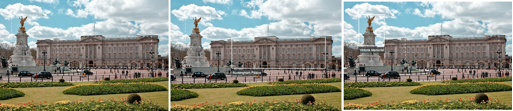
\includegraphics{images/intimage.png}
\caption{An example ``Intelligent Image'' showing the various hover over states}
\label{fig:intimage}
\end{figure}

The result of the project is that a query image is inputted, the objects contained within the image are recognised, and the image is returned with the recognised objects ``tagged'' i.e. the region of the object in the image is outlined and it can be clicked to give relevant information. In this way the standard image has been transformed into the ``intelligent image'' - one which knows about the contained scene and can offer up information to the consumer about it's contents.

Recognising a wide range of objects in an image is not a trivial problem. For such a system to be useful the following needed to be addressed:
\begin{itemize}
\item Acquire and filter enough data to create a model to perform matching on a large range of objects.
\item Create a retrieval system which provides accurate matching. False positive matching needs to be avoided as much as possible.
\item Ensure matching can be done quickly on a database of millions of objects.
\end{itemize}

To recognise millions of different objects, reference images are needed to create a model to match against. From the outset, Wikipedia\footnote{\url{http://en.wikipedia.org}} is used as the primary model data source. Wikipedia is a crowd-sourced online encyclopaedia with many images contained within the articles, and is considered an accurate source of information. In the system, each Wikipedia page defines an object, with the images in the article being used to provide the data to match against. The content of the Wikipedia article is used to give the user further information about the object. A web crawler was written to extract the relevant images of desired Wikipedia pages and create the image database. Filtering is also performed to ensure only useful images are included in the database. The data sources are fully explained in Chapter~\ref{chpt:data}.

Object retrieval uses a method employing a bag-of-words model. This builds upon the work described in x and y, more information of which is provided in Chapter~\ref{chpt:background}. The visual words in the image database from Wikipedia are precomputed. At run time, the words in the query image are computed and searched against the database of precomputed words to find the top image matches. The top matches are spatially verified, with the first verified image being the result. Subsequent improvements to the base line system (described fully in Chapter~\ref{chpt:system}) were made, including geometric improvements to the spatial verification and descriptors used to increase speed and accuracy of spatial verification, and matching improvements through query expansion using crowd-sourced data (dubbed ``Turbo-boosting'') from Microsoft's Bing\footnote{\url{http://www.bing.com}} search engine. The geometric improvements and turbo-boosting is reported in Chapter~\ref{chpt:geoimprovements} and Chapter~\ref{chpt:turboboosting} respectively.

Finally a website was developed to provide a front end interface for the system. A user can simply navigate to the website and upload an image. They then start the automatic tagging process, during which a realtime log of the process is displayed. After the query is complete, the intelligent image is displayed, which the user can interact with, see the names of the objects contained within the image, and click on the object to go to it's Wikipedia page. The software architecture of the website and the backend systems is explored in Chapter~\ref{chpt:architecture}. The result is a realtime automatic tagging system which could recognise, for example, all the buildings in a tourist's photo album of London in seconds.

The aim of the project is to work towards recognising every object on Wikipedia, however due to time restraints a subset of objects was used for development and testing of the project. The subset chosen were the pages that appear on the Wikipedia page ``List of Structures in London''\footnote{\url{http://en.wikipedia.org/wiki/List_of_structures_in_London}}.
	

%-------------------------------
% Background
%-------------------------------
\chapter{Background}
\label{chpt:background}


%-------------------------------
% Data
%-------------------------------
\chapter{Data}
\label{chpt:data}
There are three main datasets used by the application: the images from Wikipedia used to build the database of objects (Section~\ref{sec:modelimages}), the images from Microsoft Bing used for the Turbo-boosting (Section~\ref{sec:turboimages}) and the images from Google Images used for validation and testing (Section~\ref{sec:validationimages}). All images that are used are resized so that their larger dimension does not exceed 1000 pixels to reduce storage space and provide homogeneity. This chapter describes the various datasets and how they are acquired. Table~\ref{tbl:data} gives an overview of the data used.

\begin{table}[hbtp]
\begin{center}
\begin{tabular}{c|c|c|c|}
\cline{2-4}
 & Source &  \# Images &  \# Classes \\ 
 \cline{1-4}
\multicolumn{1}{|c|}{Model images} & Wikipedia & \texttt{3963} & \texttt{732} \\  
\cline{1-4}
\multicolumn{1}{|c|}{Turbo-boosting images} & Microsoft Bing & \texttt{18273} & \texttt{732} \\  
\cline{1-4}
\multicolumn{1}{|c|}{Validation images} & Google &  \texttt{701} & \texttt{294} \\  
\cline{1-4}
\end{tabular}
\end{center}
\caption{A summary of the datasets.}
\label{tbl:data}
\end{table}

\section{Model Images}
\label{sec:modelimages}
The model comprises of a dataset of images that depict the objects that are to be able to be recognised. 

Each page of Wikipedia that contains images represents an object which can be matched. The database of images which is used to build the model is simply created by visiting each page on Wikipedia for the objects desired and downloading the relevant images contained on the web page, labelling those images as being associated with the object. A script automates this process of building the model database.

\begin{figure}[htb]
\centering 
\subfloat[]{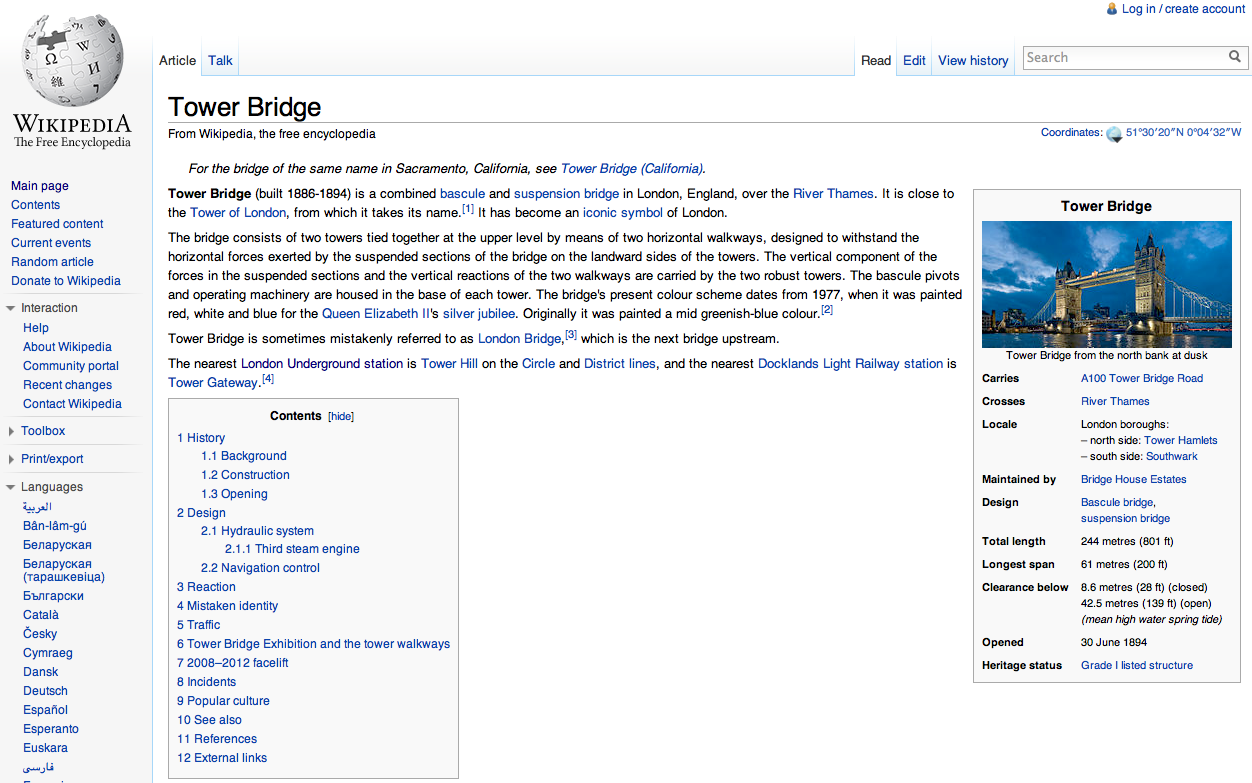
\includegraphics[width=0.5\textwidth]{images/wikipedia-article1.png}}
\subfloat[]{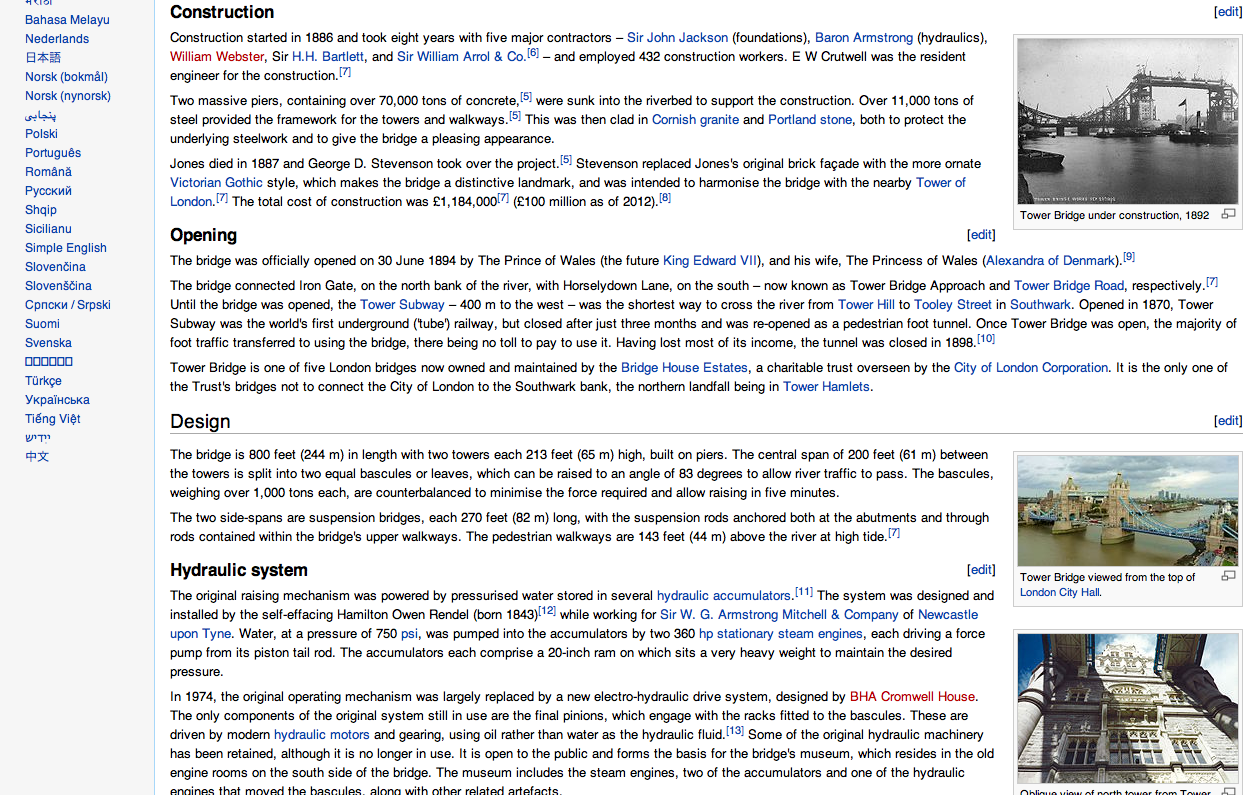
\includegraphics[width=0.5\textwidth]{images/wikipedia-article2.png}}
\caption{The Wikipedia page for ``Tower Bridge''. Note the images contained are those used in the model to represent this object.}
\label{fig:wikipage}
\end{figure}

To automate the downloading of object images from Wikipedia, Python\footnote{\url{http://www.python.org}} is used. WIkipedia offers a public application programming interface (API) over HTTP to access its data, as it is built on the MediaWiki framework\footnote{The MediaWiki framework was originally developed for Wikipedia and provides an API over HTTP as standard. \url{http://www.mediawiki.org/wiki/API} provides documentation for the API.}. However it is cumbersome and not easy to consume. Instead, a web crawler was written to explore Wikipedia pages and extract the relevant images. 

A crawler object in Python finds all the images and notes the URLs of them for subsequent download. Firstly, the HTML of the Wikipedia page must be downloaded, as it appears to a web browser (an example of a web browser being Google Chrome). However, Wikipedia does not allow crawlers and automated bots to access its web pages. To overcome this, the HTTP header\footnote{\url{http://www.w3.org/Protocols/rfc2616/rfc2616.html} describes the Hyper Text Transport Protocol and the various header fields.} of the crawler is edited to emulate that of a browser. This is implemented using the urllib2 library\footnote{\url{http://docs.python.org/library/urllib2.html}}. The code shown in Listing~\ref{lst:crawler} shows an example of how to read the HTML of the main Wikipedia homepage. The HTML document for each Wikipedia page is parsed using the BeautifulSoup library\footnote{\url{http://www.crummy.com/software/BeautifulSoup/}}. All the anchor elements are found and stored for further crawling. The images contained within the HTML are also found by looking within the part of the HTML document that is unique to the specific Wikipedia page (see Listing~\ref{lst:beautifulsoup}).

\linespread{1} % single line spacing
\lstset{language=Python,caption=The code used to gain access to Wikipedia's content using a crawler by emulating a browser.,label=lst:crawler}
\begin{lstlisting}[frame=single]
## Python
import urllib2
# Emulate the user agent as that of a browser
user_agent = "Mozilla/5.0 (Macintosh; U; Intel Mac OS X; en-US; rv:1.8.1.7) Gecko/2007091417 Firefox/2.0.0.7"
headers = {"User-Agent": user_agent}
# Request the webpage
req = urllib2.Request("http://en.wikipedia.org", headers=headers)
resp=urllib2.urlopen(req)
# Read the HTML of the response
html = resp.read()
\end{lstlisting}
\linespread{2} % double line spacing



\linespread{1} % single line spacing
\lstset{language=Python,caption=Parsing the Wikipedia article HTML document to find the relevent images.,label=lst:beautifulsoup}
\begin{lstlisting}[frame=single]
## Python
def _get_content_body(self, soup):
        main_content = soup.find('div', {"class": "mw-content-ltr"})
        if main_content is None:
            return None
        # remove navboxes
        navboxes = main_content.findAll('table', {'class': 'navbox'})
        [navbox.extract() for navbox in navboxes]
        return main_content

def _get_image_links(self, soup):
	return soup.findAll('a', {'class': 'image'})
	
# Parse the HTML
soup = BeautifulSoup(html)
# Get the main article body
soup = _get_content_body(soup)
# Get a list of image links
image_links = _get_image_links(soup)
\end{lstlisting}
\linespread{2} % double line spacing


The output of the crawler is a CSV file of the image URLs and the object class the images belong to. The object class is simply named from the URL of the Wikipedia page (for example all images appearing on \url{http://en.wikipedia.org/wiki/Tower_Bridge} will have class \lstinline!Tower_Bridge!).

The images mentioned in the CSV file produced by the crawler are then downloaded to local storage. Each image that appears on Wikipedia has a ``file page'' which displays the image along with properties and metadata on the image\footnote{For an example see \url{http://en.wikipedia.org/wiki/File:Tower_bridge_London_Twilight_-_November_2006.jpg}}. This ``file page'' is visited for each image, and the page is parsed to extract the storage URL of the image as well as its file format and original size. As the application resizes all images that exceed 1000 pixels to 1000 pixels, it is a waste of time and storage space to download the original image and later resize it. Instead, Wikipedia's inbuilt thumbnail engine is exploited, which resizes the image on Wikipedia's servers and allows you to download a thumbnail of a user selected width\footnote{\url{http://www.algorithm.co.il/blogs/programming/wikipedia-images/} describes how this is exploited}. Therefore if the original image on Wikipedia exceeds 1000 pixels, the 1000 pixel thumbnail version is downloaded instead. The images downloaded are saved in a folder named after it's class. The result is a directory containing a folder for each class, within which are the images for that class.

This process creates a structured dataset of model images from the Wikipedia pages visited. For the List of Structures in London dataset used, there were 732 classes which had 3963 images associated with them (on average 6 images per class).


\section{Turbo-boosting Images}
\label{sec:turboimages}
To achieve effective turbo-boosting, many additional images are needed to supplement the model images acquired from Wikipedia. Microsoft Bing is used as the source of the turbo-boosting images. For each class, 25 additional images are downloaded to boost that class.

Bing offers a public API that can be used to perform image searches programmatically. After obtaining an application ID from Bing for authentication, complex search requests can be made over HTTP, with the results returned in JavaScript Object Notation (JSON) format\footnote{JSON is an alternative to XML for representing structured data. \url{http://www.json.org/} provides more information.}.

Bing image search takes a number of keywords - the query - and returns a list of images from web pages related to the query. Further filters can be applied to further narrow down the search to the most relevant images. This is shown in Figure~\ref{fig:bingimages} on the website version of Bing. The ``Style'' and ``Size'' filters are especially useful in this application, as all images should be photographs for the List of Structures in London dataset, and large images are preferable so as to include as much detail as possible. Setting these filters precludes many instances of graphics and logos which are not suitable for turbo-boosting.

\begin{figure}[htb]
\centering 
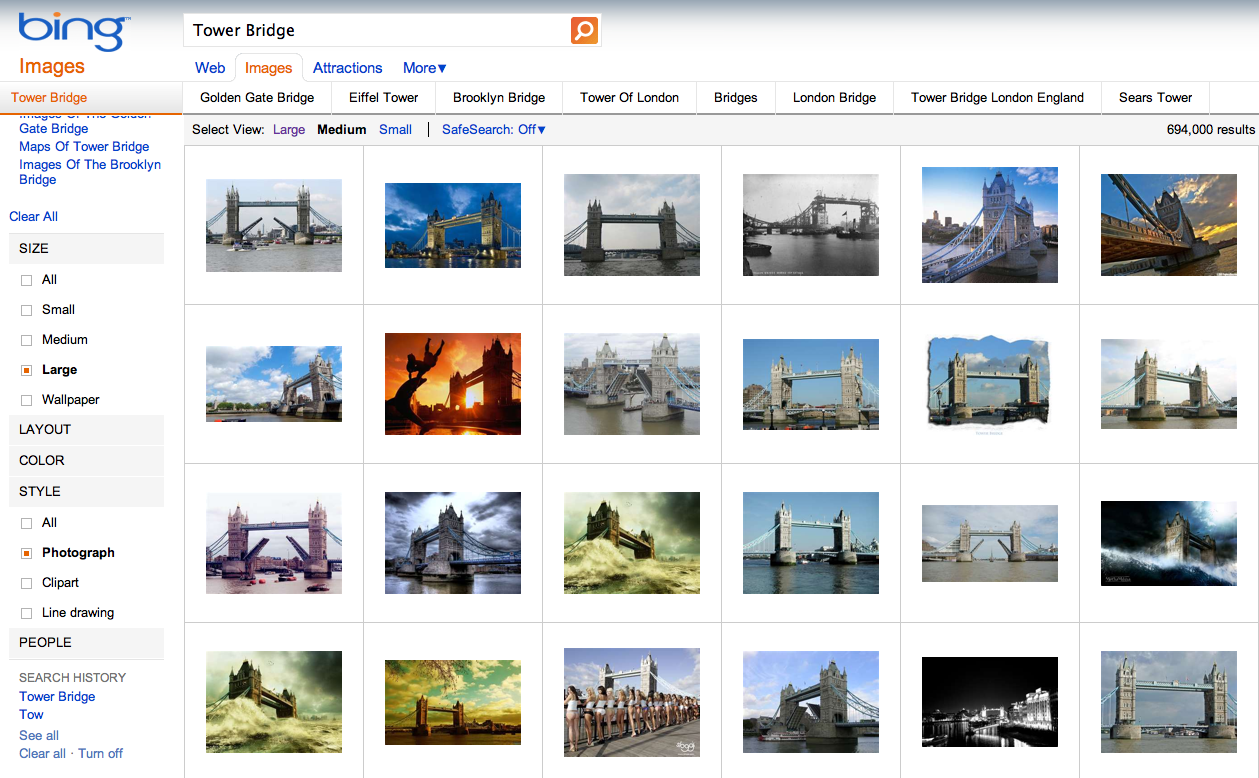
\includegraphics[width=0.9\textwidth]{images/bing-images.png}
\caption{The browser interface of Bing image search which is replicated in the API query URL. Note the filters in the left column.}
\label{fig:bingimages}
\end{figure}

All the parameters that appear in the web interface for Bing image search can be replicated in the API request with query parameters. A MATLAB script is used to consume the API and download the images. Listing~\ref{lst:bingapi} shows the URL used for the API call to get the search results for the images for a particular class. The URL encoded\footnote{URL encoding ensures that all characters are in a form which can be used as a URL. See \url{http://www.w3schools.com/tags/ref_urlencode.asp} for more information.} class name is used as the query. For example, for the class \lstinline!Tower_Bridge!, the variable \lstinline!search_term! appearing in Listing~\ref{lst:bingapi} will be set to \lstinline!"Tower%20Bridge"! (note \lstinline{" "} is URL encoded as \lstinline{"%20"}). Both the ``Style'' and ``Size'' image filters are set to ``Photo'' and ``Large'' respectively by setting the \lstinline!Image.Filters! parameter.

\linespread{1} % single line spacing
\lstset{language=Matlab,caption=A Bing image search API request.,label=lst:bingapi}
\begin{lstlisting}[frame=single]
%% MATLAB
request_url = ['http://api.bing.net/json.aspx?' ...
                   'AppId=' app_id ...
                   '&Query=' search_term ...
                   '&Sources=Image' ...
                   '&Version=2.0' ...
                   '&Adult=Strict' ...
                   '&Image.Count=' nPhotos ...
                   '&Image.Filters=Style:Photo+Size:Large' ...
                   '&JsonType=raw' ...
                  ];
% Read the result of the request
response = urlread(request_url);
% Parse the result from JSON to MATLAB structure form
resp_struct = parse_json(response);
\end{lstlisting}
\linespread{2} % double line spacing

Using MATLAB's inbuilt \lstinline!urlread! function, the search results are requested and returned in JSON format. The JSON result is then parsed and converted into a MATLAB structure object for reading. An example JSON response is shown in Listing~\ref{lst:bingjson}. Each element in the array \lstinline!Results! is an image result. Each image is then downloaded from its \lstinline!MediaUrl! field using a modified version of the \lstinline!imread! function which allows for request timeouts, as some image resources may have expired since their submission to the Bing database.

\linespread{1} % single line spacing
\lstset{language=Java,caption=A Bing image search response in JSON format. The ``Results'' array is truncated to one element.,label=lst:bingjson}
\begin{lstlisting}[frame=single]
// JSON
{
   "SearchResponse":{
      "Version":"2.0",
      "Query":{
         "SearchTerms":"Tower Bridge"
      },
      "Image":{
         "Total":780000,
         "Offset":0,
         "Results":[
            {
               "Title":"Tower Bridge - London Photo (551176) - Fanpop",
               "MediaUrl":"http://images.fanpop.com/images/image_uploads/Tower-Bridge.jpg",
               "Url":"http://www.fanpop.com/spots/london/images/551176/title/tower-bridge",
               "DisplayUrl":"http://www.fanpop.com/spots/london/images/title/tower-bridge",
               "Width":1600,
               "Height":1200,
               "FileSize":761104,
               "Thumbnail":{
                  "Url":"http://ts3.mm.bing.net/images/thumbnail.aspx?q=4757...",
                  "ContentType":"image/jpeg",
                  "Width":160,
                  "Height":120,
                  "FileSize":3274
               }
            }, ...
         ]
      }
   }
}
\end{lstlisting}
\linespread{2} % double line spacing

The downloaded images are resized if larger than 1000 pixels and stored in a folder named after its class. As for the model images, the result is a directory containing a folder for each class, within which are the turbo-boosting images for that class.

\section{Validation Images}
\label{sec:validationimages}

Images are needed to test and validate the yield performance of the object recognition system. Therefore a separate dataset of images with their ground truth classes is needed. Ideally all classes would be tested and each test image should be a fair representation of the object of that class. Google image search was used first to automatically download 8 images for each class. The images were then checked manually to refine the dataset.

Google image search is very similar to Bing image search described in the previous section. However the results are markedly different, providing another set of images that are perfect for testing. Google offers an API over HTTP which can be used to search based on a text query and, as with Bing, filters can be applied. The result is returned in JSON format.

\linespread{1} % single line spacing
\lstset{language=Matlab,caption=A Google image search API request.,label=lst:googleapi}
\begin{lstlisting}[frame=single]
%% MATLAB
request_url = ['https://ajax.googleapis.com/ajax/services/search/images?v=1.0' ...
	'&q=' search_term ...
	'&as_filetype=jpg' ...
	'&imgsz=xxlarge' ...
	'&imgtype=photo' ...
	'&rsz=8' ...
];
% Read the result of the request
response = urlread(request_url);
% Parse the result from JSON to MATLAB structure form
resp_struct = parse_json(response);
\end{lstlisting}
\linespread{2} % double line spacing

Listing~\ref{lst:googleapi} shows the formulation and request of a Google search API request. As with the Bing requests, the search term is the URL encoded class name. The JSON response (Listing~\ref{lst:googlejson}) is parsed into a MATLAB object and the \lstinline!url! field is used to download the image.

\linespread{1} % single line spacing
\lstset{language=Java,caption=A Google image search response in JSON format. The ``results'' array is truncated to one element.,label=lst:googlejson}
\begin{lstlisting}[frame=single]
// JSON
{
   "responseData":{
      "results":[
         {
            "GsearchResultClass":"GimageSearch",
            "width":"1024",
            "height":"819",
            "imageId":"ANd9GcSTU9Qv93OE3Q5kjo0h5Dcsl6sYBGURxSlmw8tfUbISx6heecXcY9VKkquZ",
            "tbWidth":"150",
            "tbHeight":"120",
            "unescapedUrl":"http://www2.hiren.info/desktopwallpapers/natural/the-tower-...",
            "url":"http://www2.hiren.info/desktopwallpapers/natural/the-tower-bridge.jpg",
            "visibleUrl":"www.hiren.info",
            "title":"Desktop Wallpapers � Natural Backgrounds � The \u003cb\u003eTower Bridge\u003c/b\u003e \u003cb\u003e...\u003c/b\u003e",
            "titleNoFormatting":"Desktop Wallpapers � Natural Backgrounds � The Tower Bridge ...",
            "originalContextUrl":"http://www.hiren.info/desktop-wallpapers/natural-pic...",
            "content":"The \u003cb\u003eTower Bridge\u003c/b\u003e, London,",
            "contentNoFormatting":"The Tower Bridge, London,",
            "tbUrl":"http://t1.gstatic.com/images?q\u003dtbn:ANd9GcSTU9Qv93OE3Q5kjo..."
         }, ...
      ], ...
   "responseDetails":null,
   "responseStatus":200
}
\end{lstlisting}
\linespread{2} % double line spacing

As with the turbo-boosting images, the downloaded images are resized if larger than 1000 pixels stored in a folder named after its class. Again, the result is a directory containing a folder for each class, within which are the turbo-boosting images for that class.

After automatic download of potential test images for each class, the dataset was checked over manually. Images that appear in the model dataset, as well as images that do not fairly depict the class they are to test are removed from the test set . 

%-------------------------------
% Baseline system
%-------------------------------
\chapter{Baseline system}
\label{chpt:system}
The base line system draws upon the research and literature mentioned in Chapter~\ref{chpt:background}. Upon starting the project, an application was provided that includes a basic database creation and image matching process based on a dataset of structures in Oxford. This application was expanded upon to create the current system.

There are two separate processes which form the project. The first is the pre-computation process that creates the databases and data structures required for object recognition. The second is the object recognition process that takes a query image and returns the names and locations of the objects in the image. A summary of these two processes is described in Figure~\ref{fig:precompprocess} and Figure~\ref{fig:searchprocess} respectively.

\begin{figure}[htb]
\centering 
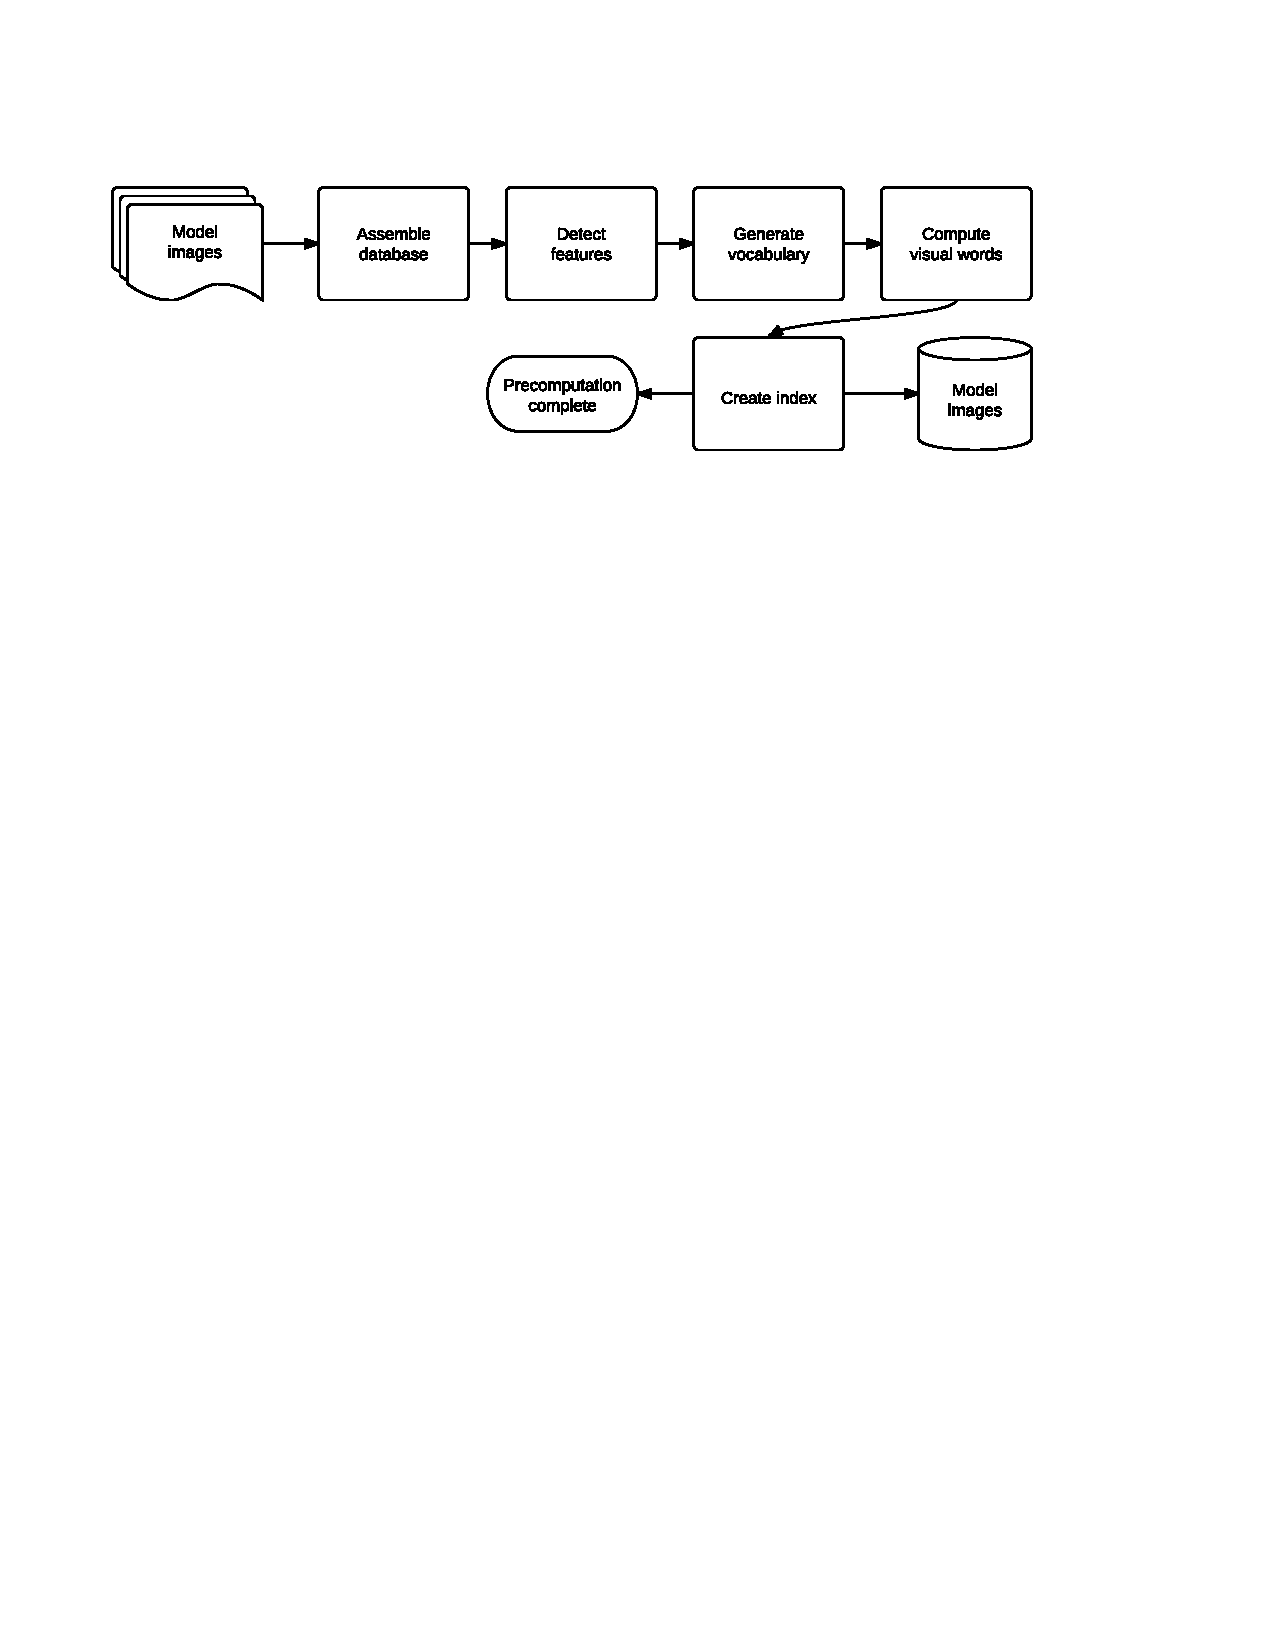
\includegraphics[width=0.6\textwidth]{images/PrecomputeProcess.pdf}
\caption{The flow diagram for the basic pre-computation process.}
\label{fig:precompprocess}
\end{figure}

\begin{figure}[htb]
\centering 
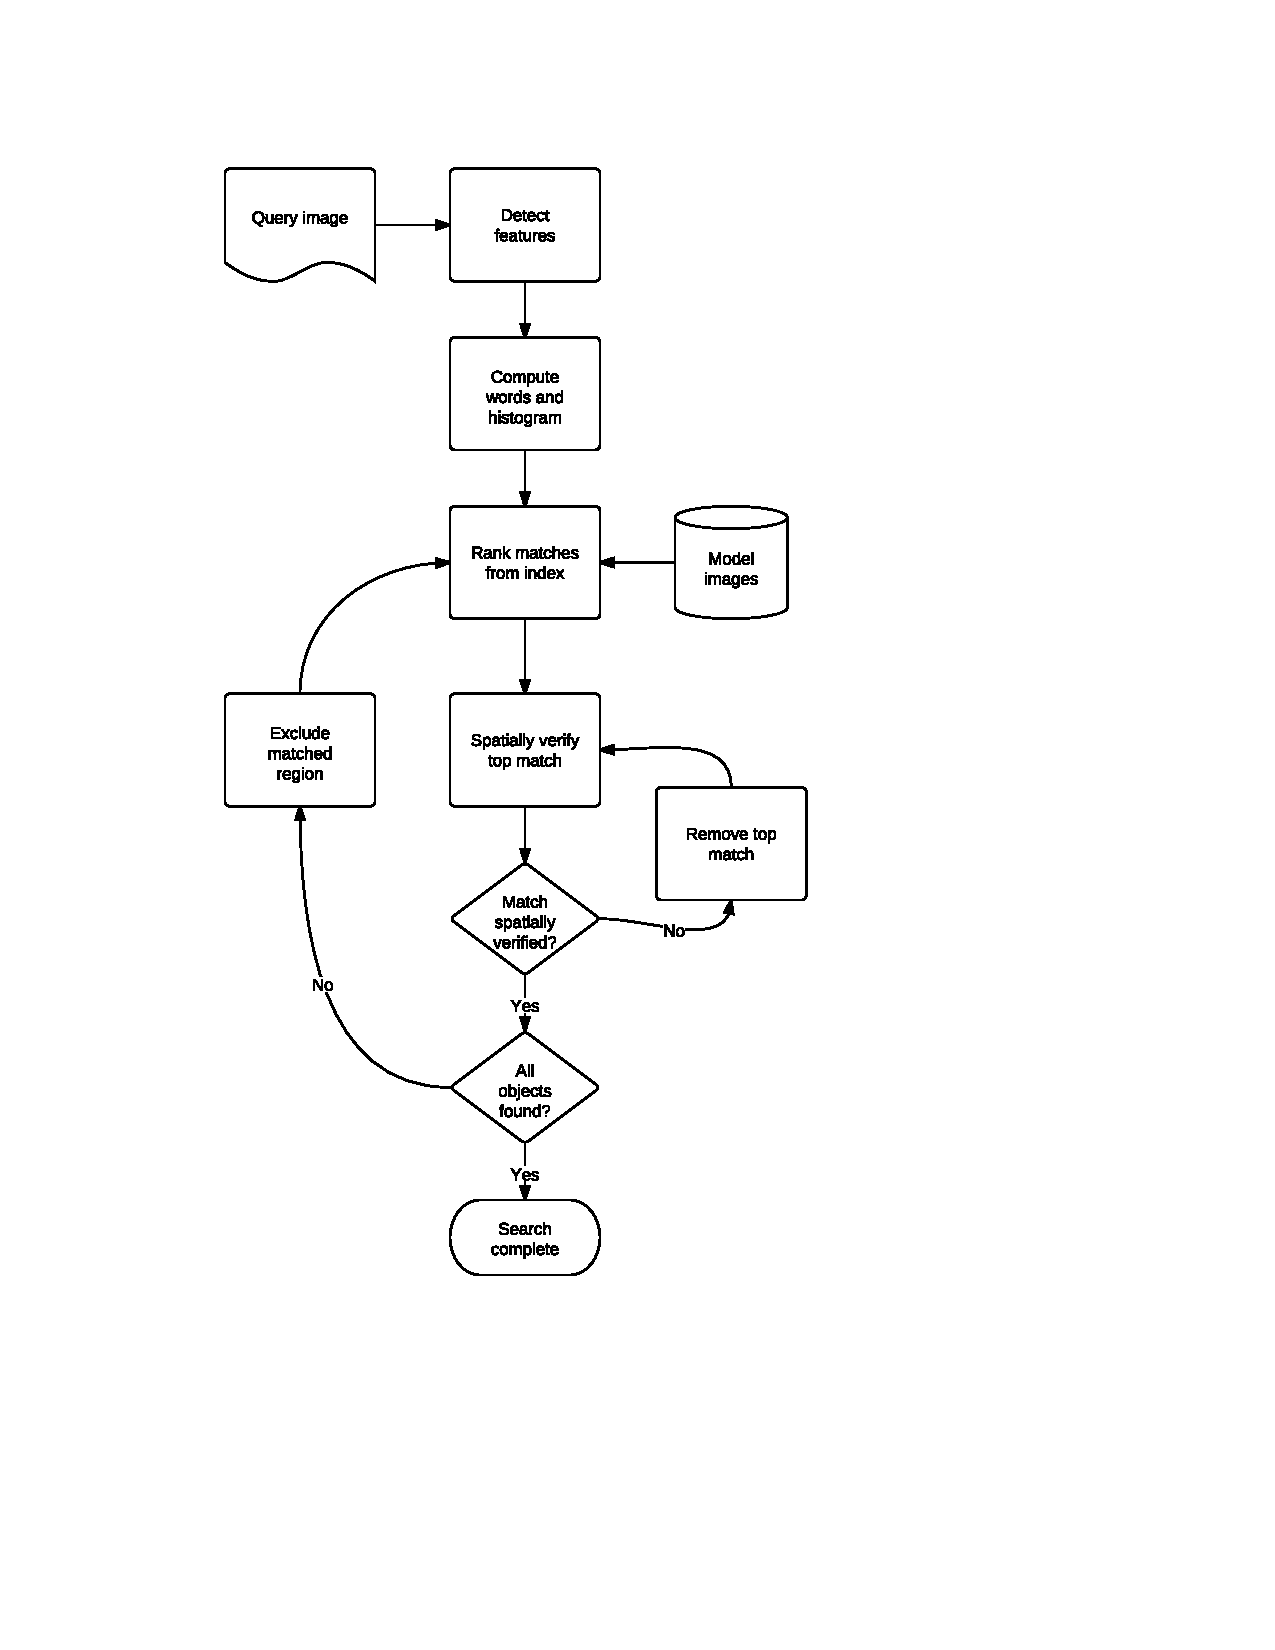
\includegraphics[width=0.5\textwidth]{images/SearchProcess.pdf}
\caption{The flow diagram for the basic object recognition process.}
\label{fig:searchprocess}
\end{figure}

The pre-computation process is run once on the dataset to produce the database and working data structures required for the object recognition process. For each model image, the features are detected and associated descriptors generated. This is described further in Section~\ref{sec:featuredetection}. A sample of the features are then used to generate the visual word vocabulary (Section~\ref{sec:visualwords}). The histograms of visual words are then weighted and collected into an index ready for querying (Section~\ref{sec:histograms}). This completes the basic pre-computation process and the system is ready for use.

The object recognition process takes a query image and attempts to recognise the objects contained within the image. Firstly, the feature descriptors are computed for the detected features within the query image. The visual words are computed based on the vocabulary created during the pre-computation process, and the weighted histogram produced for the query image. A search is then performed on the index of histograms for the model images (see Section~\ref{sec:histograms}) the output of which is a list of images based on how highly they match the query image. Going down the list of top matches by histogram, spatial verification is performed to ensure the visual words in both the query image and match image form the same shaped object (all objects are assumed rigid). This is described in Section~\ref{sec:spatialverification}. Once a match has been spatially verified, this object is deemed recognised and added to the list of found objects. Multiple matching is then performed by repeating this process, excluding regions of the image containing a previously recognised object (Section~\ref{sec:multiobject}).

The remainder of this chapter describes further details of the parts of the processes described above.

\section{Feature Detection and Description}
\label{sec:featuredetection}
The feature detection and description methods used are the original scale-invariant feature transform (SIFT) algorithms. The advantages of using SIFT are that the detected features and their descriptors are invariant to image translation, scaling, and rotation, partially invariant to illumination changes and robust to local geometric distortion. This is essential to be able to match the same object features across varied sources of images.

The SIFT features are defined as maxima and minima of the result of difference of Gaussians function\footnote{\url{http://en.wikipedia.org/wiki/Difference_of_Gaussians}} applied in scale-space to a series of smoothed and resampled images. Low contrast candidate points and edge response points along an edge are discarded. These features are then described by the SIFT feature descriptor - a 128-dimensional vector.

The result of the SIFT feature detection and description algorithm are two matrices. The first is a matrix of feature points or frames, Equation~\ref{eqn:frames}, where each column describes the position $(x_i, y_i)$ in the image, the scale $s_i$ and orientation $\theta_i$ for feature $i$. Corresponding to the frames matrix is a descriptor matrix, Equation~\ref{eqn:descrs}, where each column is the 128-D vector $\mathbf{d_i}$ that describes feature $i$.

\begin{equation}
\left[ \begin{array}{ccccc}
x_1 & x_2 & \cdots & x_{N-1} & x_N \\
y_1 & y_2 & \cdots & y_{N-1} & y_N \\
s_1 & s_2 & \cdots & s_{N-1} & s_N \\
\theta_1 & \theta_2 & \cdots & \theta_{N-1} & \theta_N
\end{array}\right]
\label{eqn:frames}
\end{equation}

\begin{equation}
\left[ \begin{array}{ccccc}
\mathbf{d_1} & \mathbf{d_2} & \cdots & \mathbf{d_{N-1}} & \mathbf{d_N} 
\end{array}\right]
\label{eqn:descrs}
\end{equation}

\section{Visual Words}
\label{sec:visualwords}
To avoid matching features in unbounded, 128-dimensional space, the SIFT features are quantised. These quantised SIFT features are known as visual words.

During the pre-computation process, the vocabulary of words is created. The vocabulary is essentially the clustering of SIFT space. The number of clusters (visual words) to be created is the vocabulary size, 100,000 for this application. Vocabulary creation is done using the approximate nearest neighbours K-means algorithm. The clustering is performed on a random sample from all the feature descriptors for the entire model images dataset. The number of features sampled was 30 times the size of the vocabulary, i.e. 3 million. 

The result of the vocabulary creation is a kd-tree which can be used to get the word associated with a SIFT descriptor. Each word is assigned an ID, and the images can then be represented as a list of words, where each word is the nearest visual word to the SIFT descriptor.

\section{Histograms and Index}
\label{sec:histograms}
The images are represented by a list of words as described in the previous section. This list of words can in turn be represented as a histogram, with each element containing the number of occurrences of the word with ID equal to the element number in the image. Therefore each histogram is a sparse 100,000 element array. Two examples of the raw histograms are shown in Figure~\ref{fig:rawhist1} and Figure~\ref{fig:rawhist2}.

The term frequency-inverse document frequency\footnote{\url{http://en.wikipedia.org/wiki/Tf*idf}} (tf-idf) weights are then computed for each word across the entire dataset of model images. These weights are applied to the histograms to down-weight common, uninformative visual words and up-weight unique, informative visual words. The differences in histograms before and after weighting is illustrated in Figure~\ref{fig:histograms}.

\begin{figure}[htb]
\centering 
\subfloat[Tower Bridge image 1]{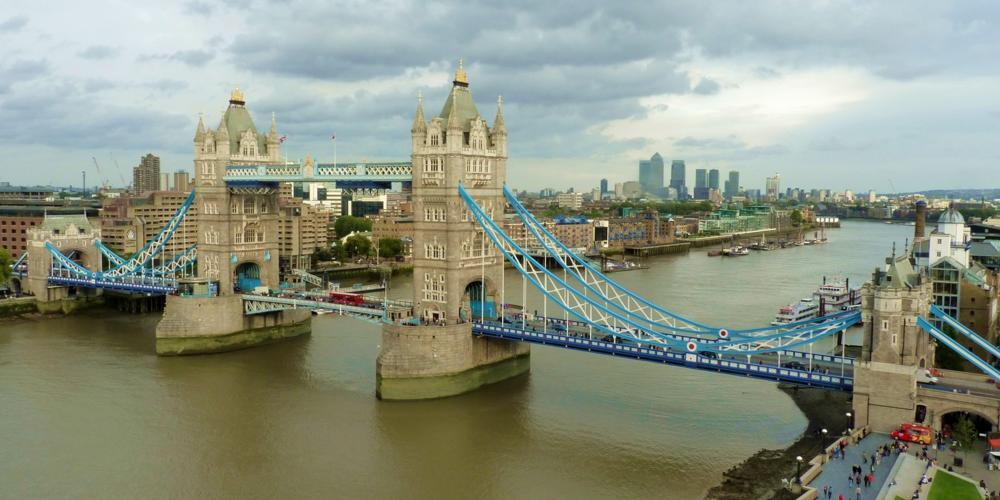
\includegraphics[width=0.4\textwidth]{images/tb_city_hall.jpg}}
~
\subfloat[Tower Bridge image 2]{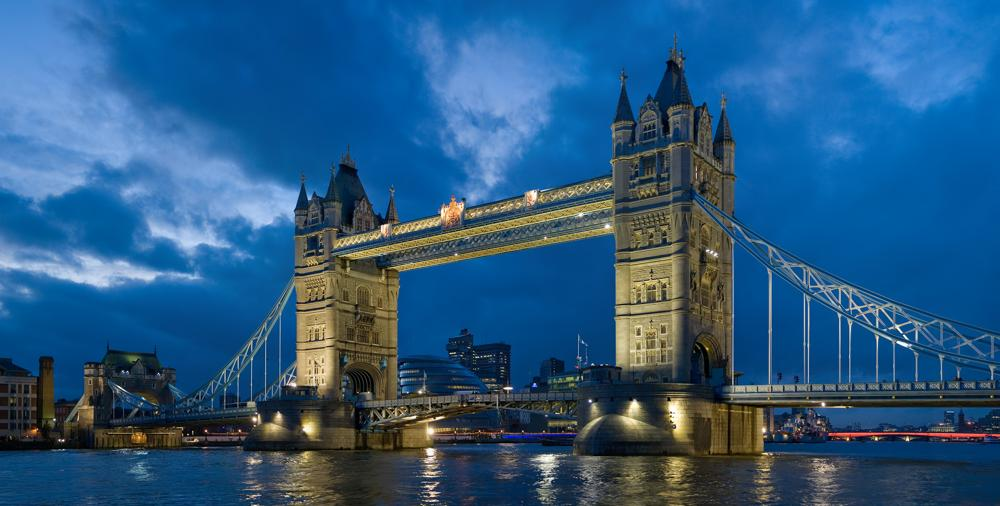
\includegraphics[width=0.4\textwidth]{images/tb_twilight.jpg}}
\\
\subfloat[Raw histogram for image 1]{\label{fig:rawhist1}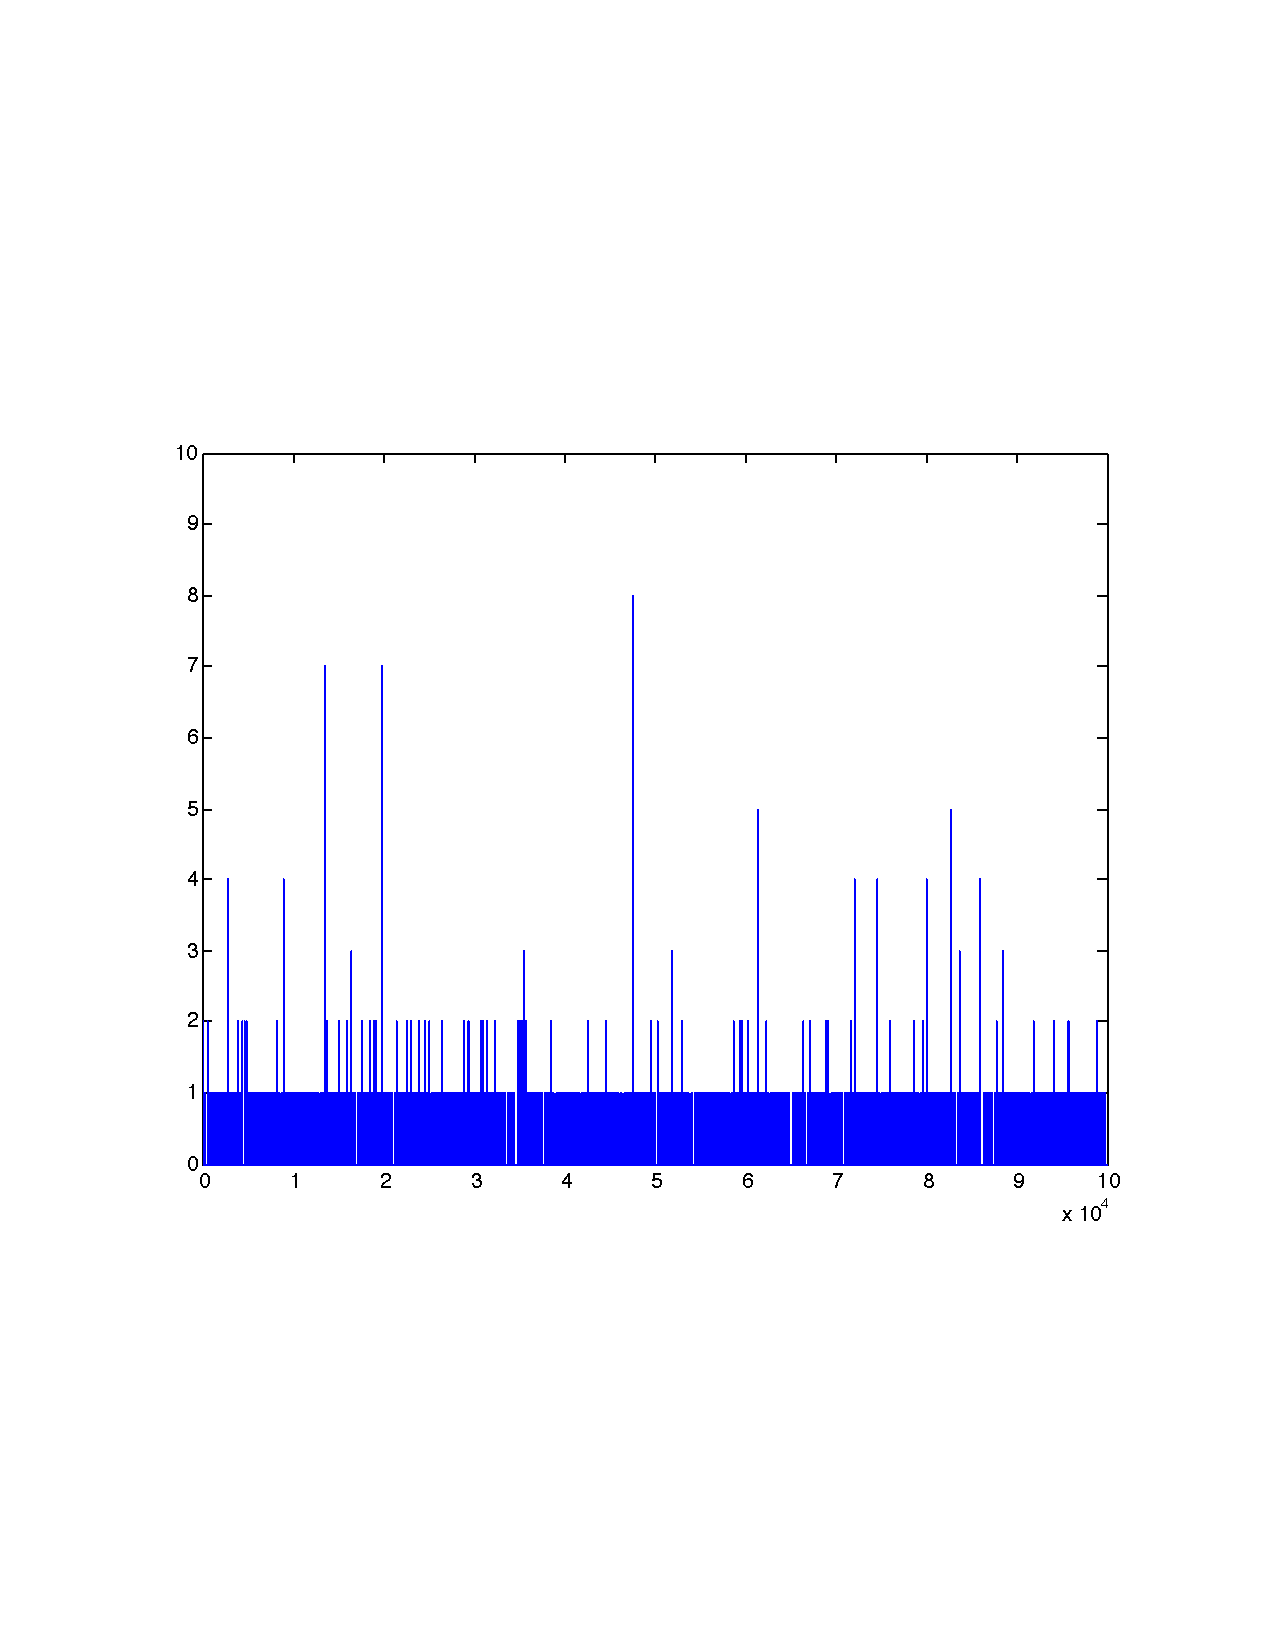
\includegraphics[width=0.4\textwidth]{images/tb_city_hall.pdf}}
~
\subfloat[Raw histogram for image 2]{\label{fig:rawhist2}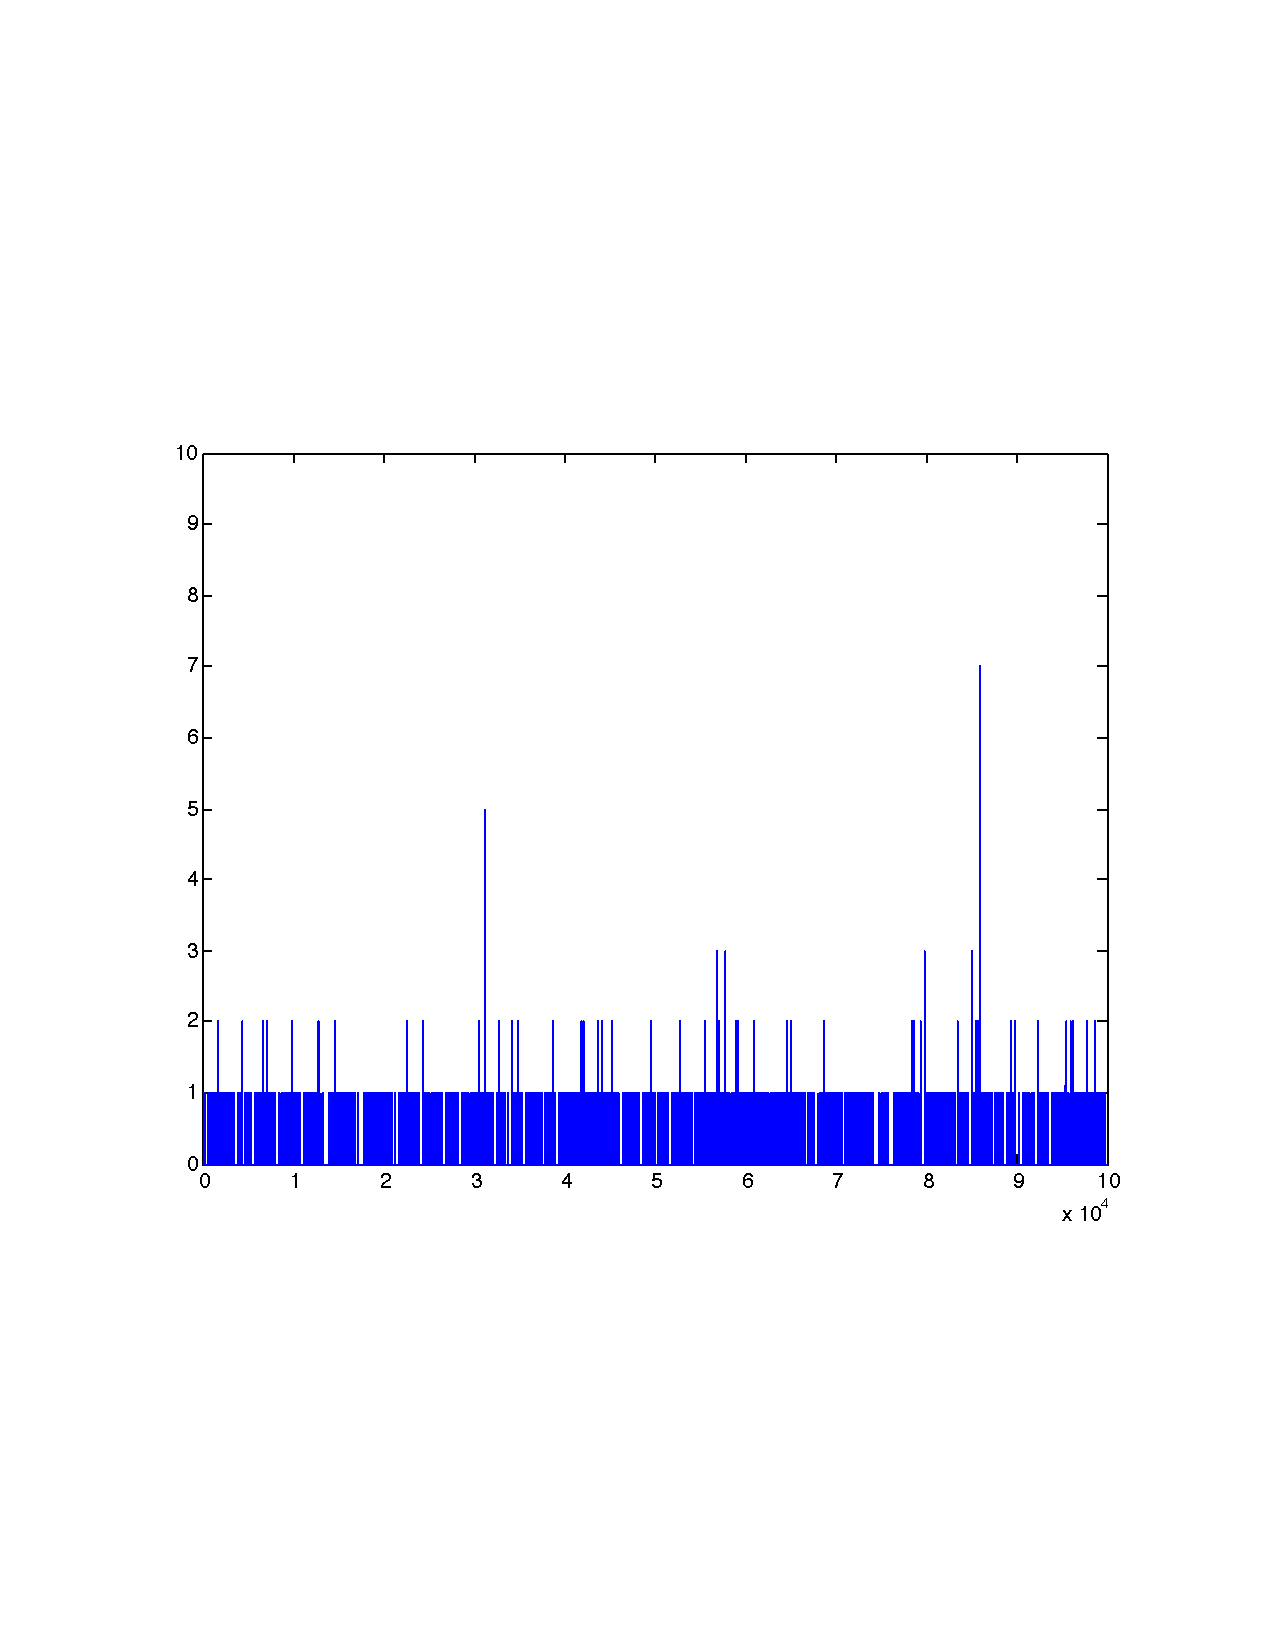
\includegraphics[width=0.4\textwidth]{images/tb_twilight.pdf}}
\\
\subfloat[Weighted histogram for image 1]{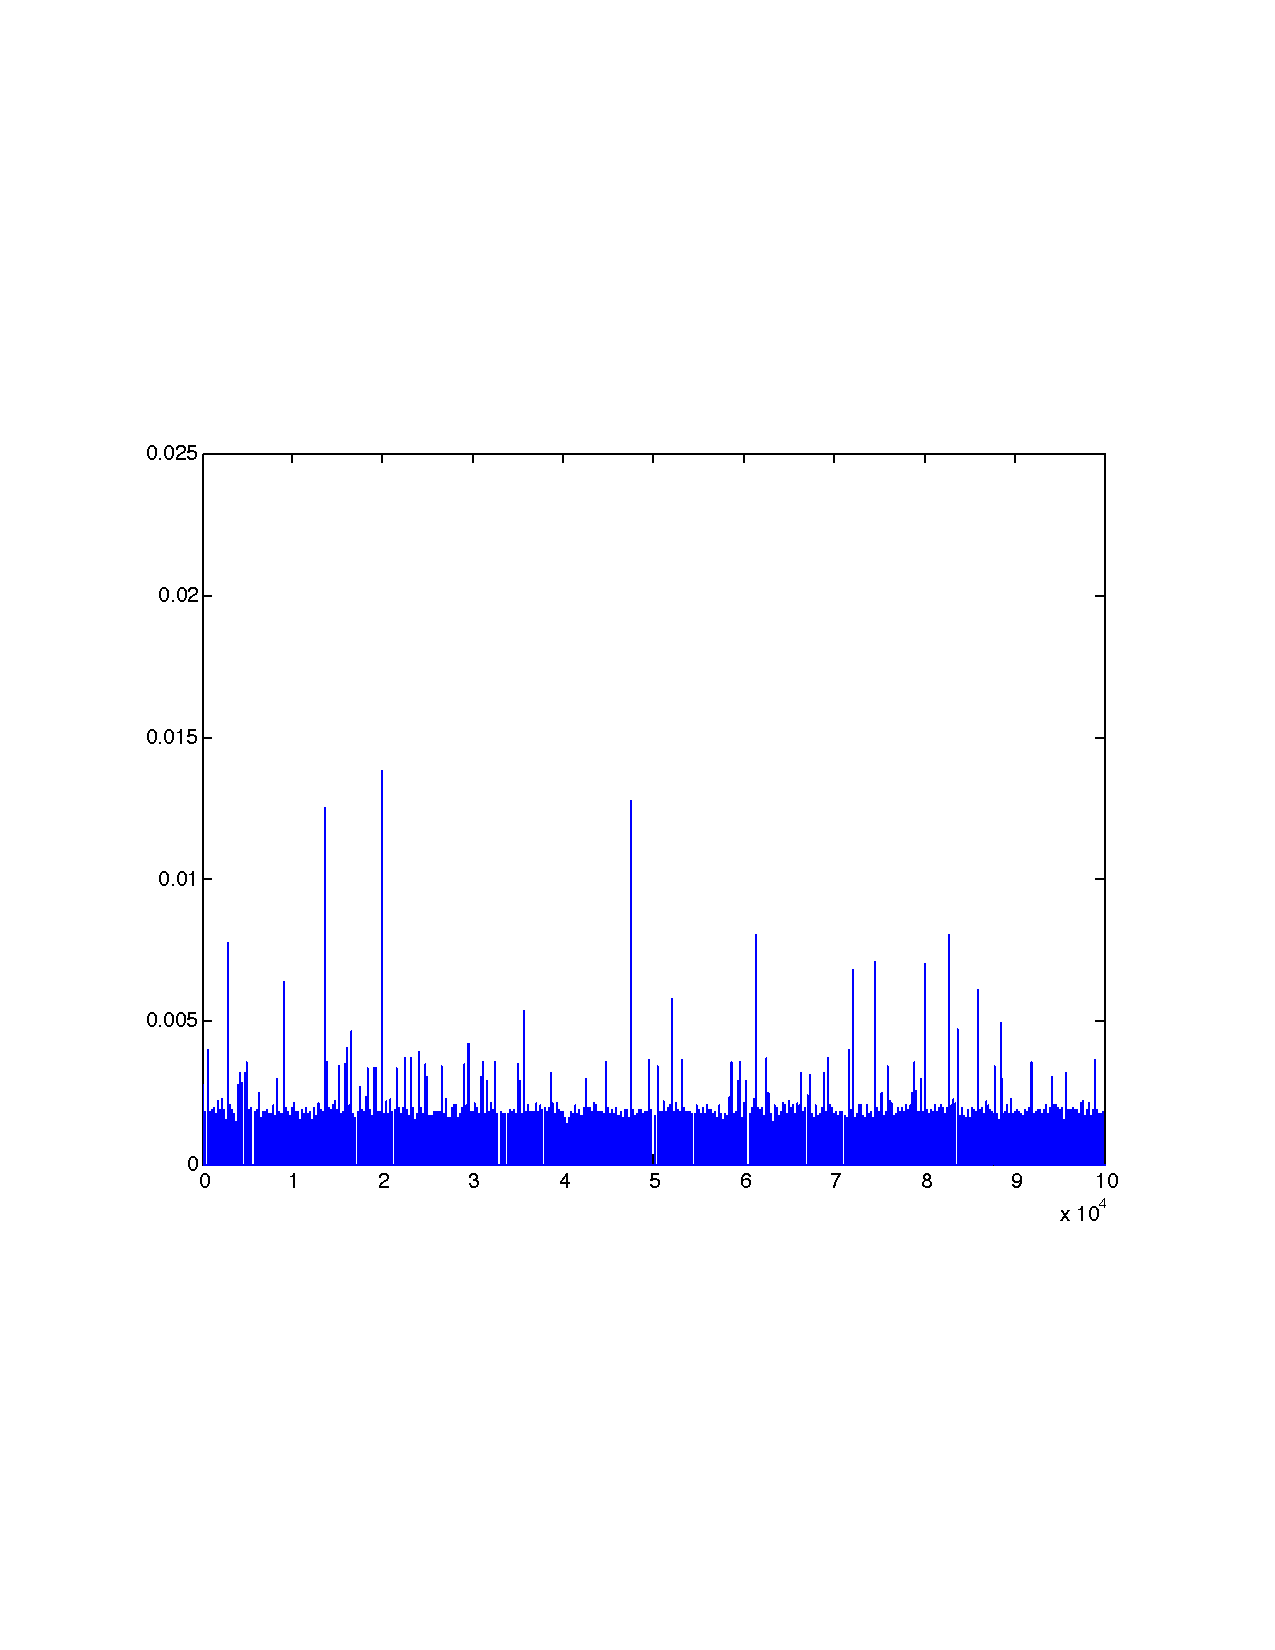
\includegraphics[width=0.4\textwidth]{images/tb_city_hall_weighted.pdf}}
~
\subfloat[Weighted histogram for image 2]{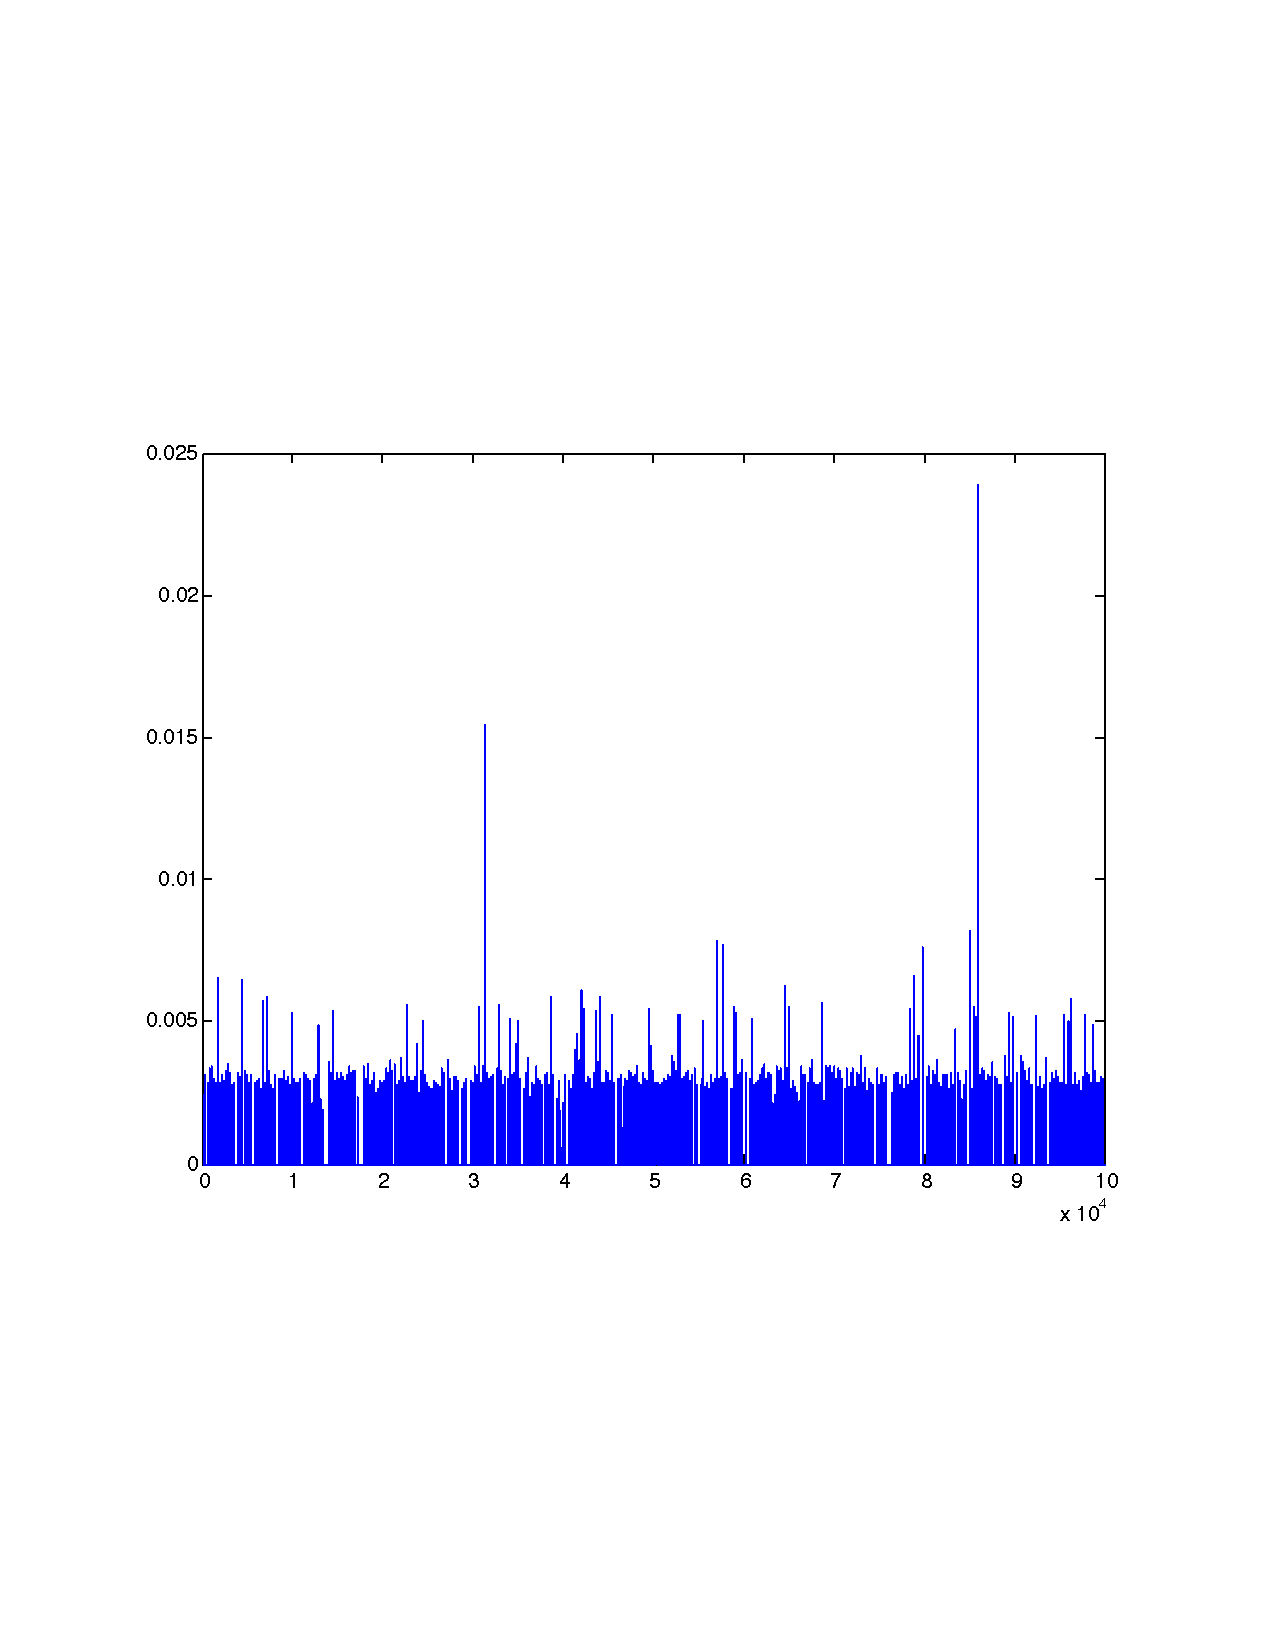
\includegraphics[width=0.4\textwidth]{images/tb_twilight_weighted.pdf}}
\caption{Two images for the class \lstinline!Tower_Bridge! with their raw histograms and tf-idf weighted histograms}
\label{fig:histograms}
\end{figure}

Each model image therefore has a histogram that is used for matching. All the histograms are packaged into a matrix (each column being an image's histogram) that is used as the index for query matching.

To find the most similar images to a query image, a dot product is performed between each of the model image histograms and the query image histogram. This is shown in Equation~\ref{eqn:tfidfscore}, where $\mathbf{h_{query}}$ is the tf-idf weighted histogram of the query image and $\mathbf{h_i}$ is the tf-idf weighted histogram of model image $i$. $\mathbf{scores}$ is a $Nx1$ array with the result of the dot product with each model image's histogram in each element. The matches are ranked in decreasing order of their score - the model image with the highest score said to be the most similar to the query image.

\begin{equation}
\mathbf{scores}= \mathbf{h_{query}^T}
\left[ \begin{array}{ccccc}
\mathbf{h_1} & \mathbf{h_2} & \cdots & \mathbf{h_{N-1}} & \mathbf{h_N}
\end{array}\right]
\label{eqn:tfidfscore}
\end{equation} 


\section{Spatial Verification}
\label{sec:spatialverification}
Matching based purely on the tf-idf weighted histograms is effective, however it is prone to false positives. This is due to the fact that two different objects may have very similar features (and therefore many similar visual words), but these features are in very different places as they are not the same object. Therefore, a final spatial verification must be done to ensure that the visual words that appear both in the query image and the model image form the same rigid bodied object.

The spatial verification restraint in this application is that there should exist an affine transformation\footnote{\url{http://en.wikipedia.org/wiki/Affine_transformation}} between the scene in the query image and the scene in model image that is the potential match. Practically, this means that there should be an affine transformation that maps the visual words in the query image to the position of the same visual words in the model image.

The random sample consensus algorithm\footnote{\url{http://en.wikipedia.org/wiki/RANSAC}} (RANSAC) is used to estimate an affine transformation between the two images, using the corresponding visual words in each image. The result of the RANSAC spatial verification is the number of visual words in the query image that map to the correct positions in the model image (within some tolerance region). Matches that have enough inliers under the transformation are said to be spatially verified - that is the estimated affine transformation is accurate and both images depict the same rigid bodied object.

Figure~\ref{fig:spatialverification} shows the result of spatial verification on matched SIFT features. Note the disregarding of some matches after RANSAC as these matches do not conform with the estimated affine transformation.

\begin{figure}[htb]
\centering 
\subfloat[Big Ben image 1]{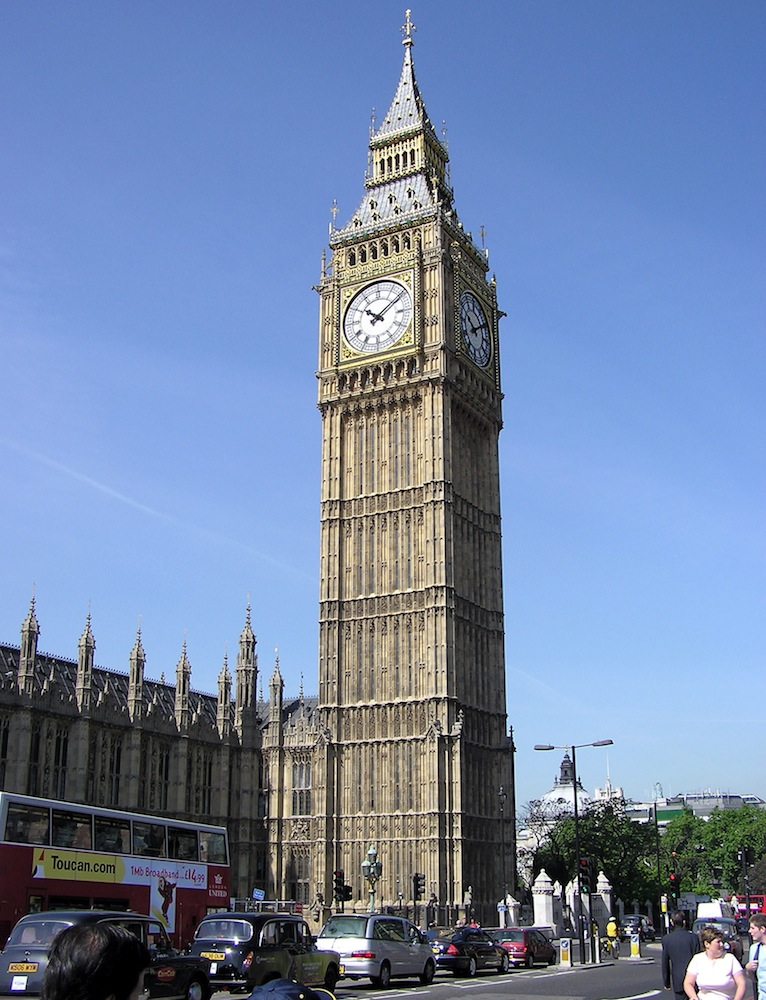
\includegraphics[width=0.3\textwidth]{images/bigben.jpg}}
~
\subfloat[Big Ben image 2]{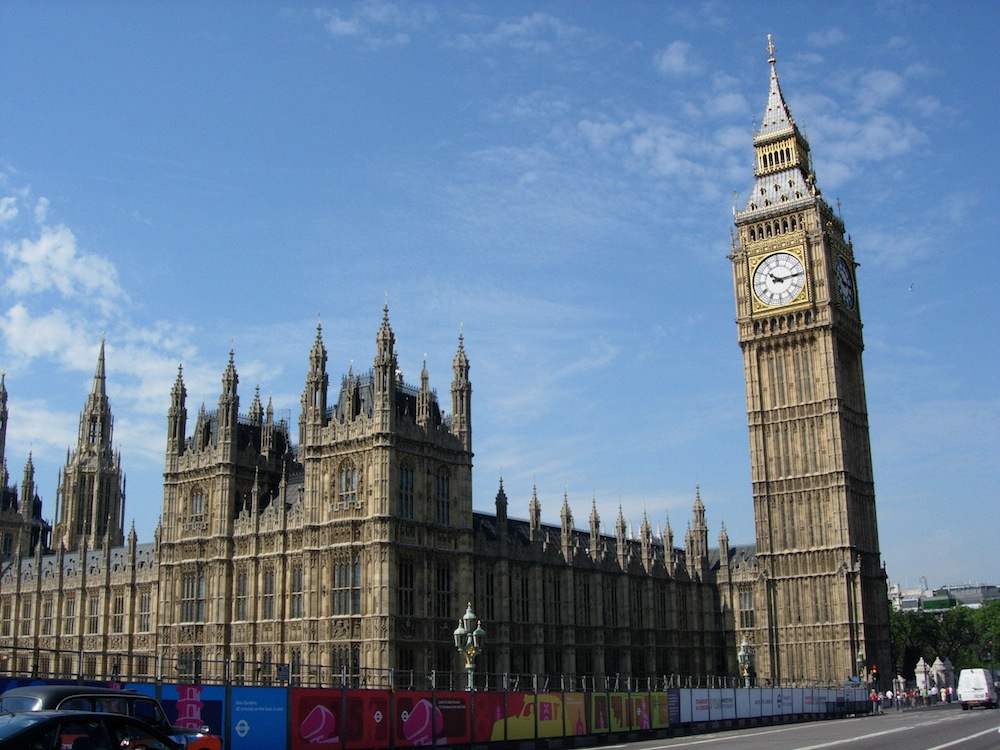
\includegraphics[width=0.3\textwidth]{images/bigben2.jpeg}}
\\
\subfloat[Matches based purely on SIFT feature similarity]{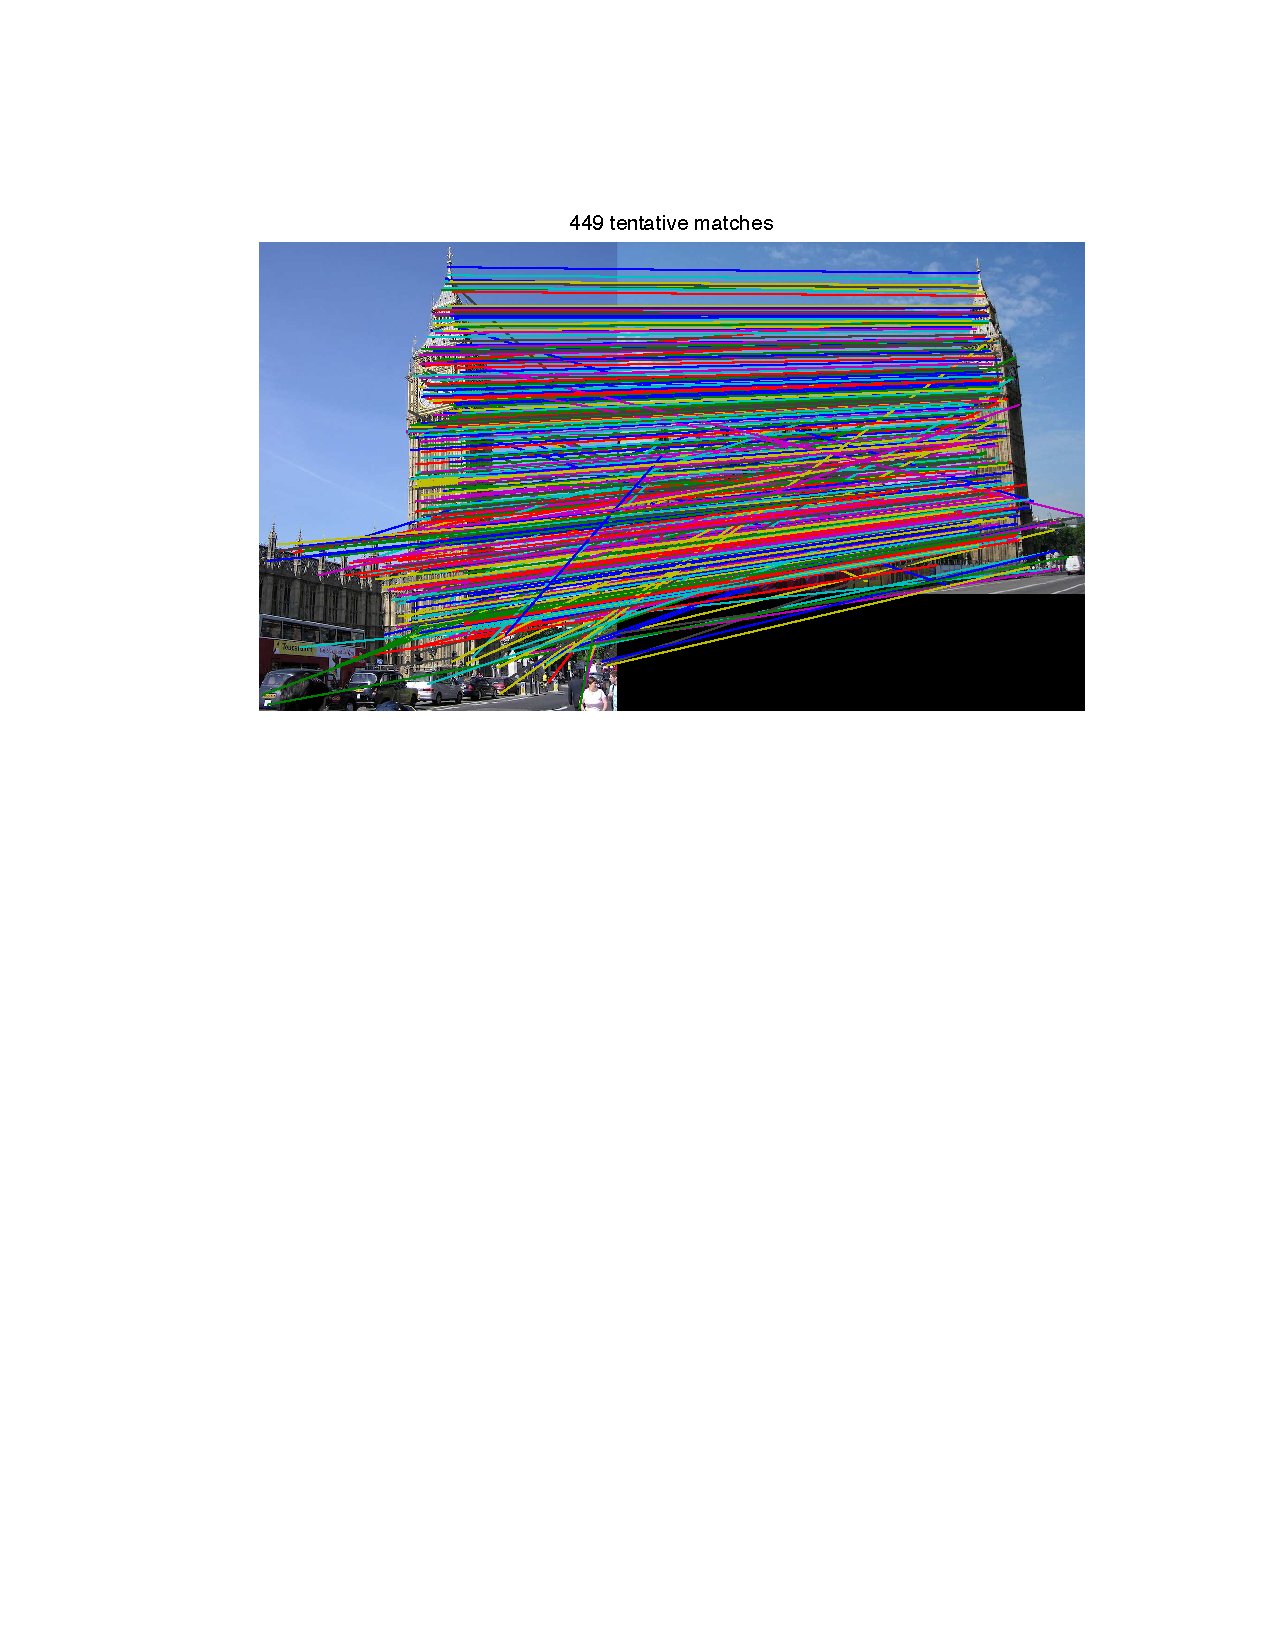
\includegraphics[width=0.5\textwidth]{images/spatial_verification1.pdf}}
\subfloat[Matches after RANSAC spatial verification]{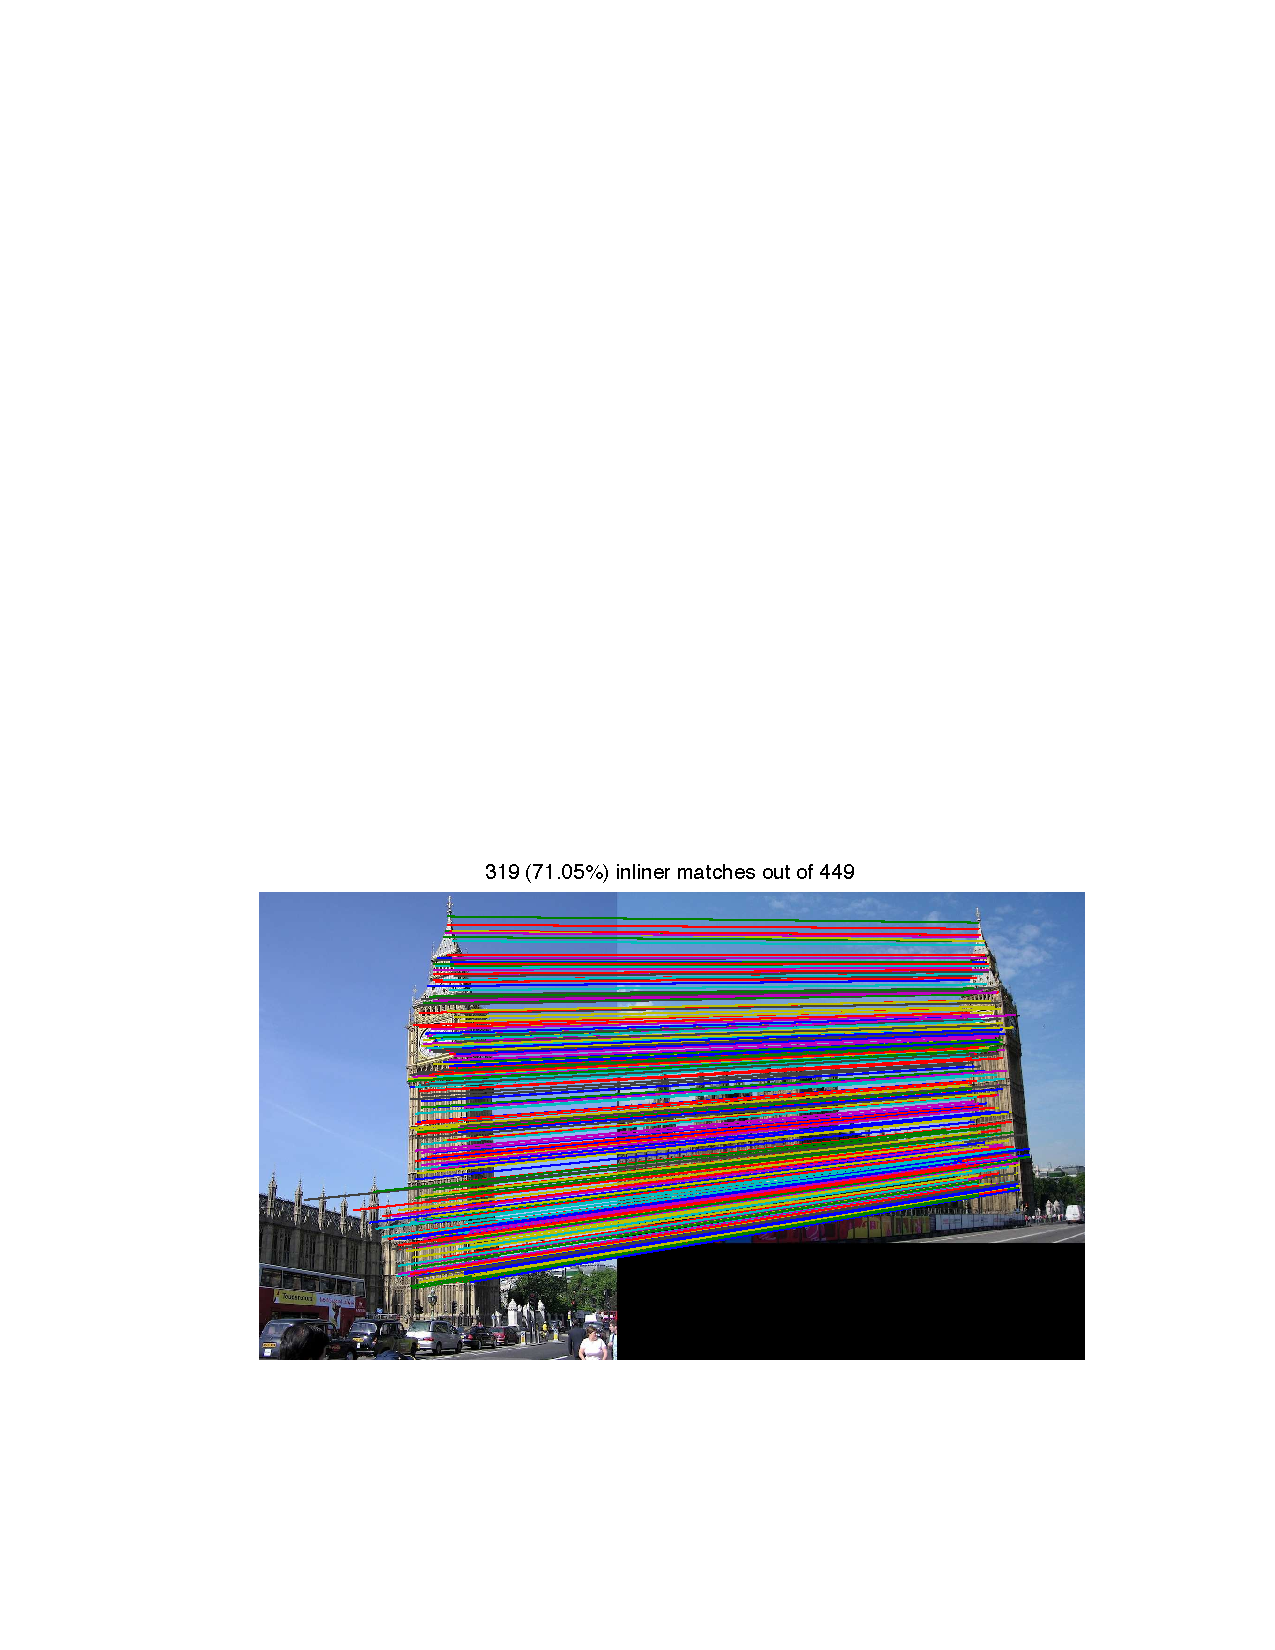
\includegraphics[width=0.5\textwidth]{images/spatial_verification2.pdf}}
\caption{RANSAC spatial verification performed on two images of Big Ben.}
\label{fig:spatialverification}
\end{figure}

Spatial verification is performed on each model image in descending order of the tf-idf histogram matching score. The first model image to be successfully spatially verified is deemed to be an accurate match and the process is terminated, with the class the model image represents being the object found. The region of the query image that is labelled as the object is the bounding box of visual words that spatially match the model image.


\section{Multiple Object Matching}
\label{sec:multiobject}
The object recognition engine can recognise multiple objects in a single image (an example is shown in Figure~\ref{fig:multiplematching}). Once an object has been successfully recognised, the query is re-issued with the same query image, however the visual words contained within the regions of already recognised objects are excluded from the query process. Previously recognised objects are ignored as matches from the re-issued queries and the process finishes when no new objects can be found. 

This method allows any number of objects to be recognised within a single image. The downside of this process is that it requires multiple queries so increases the time taken to complete.

\begin{figure}[htb]
\centering 
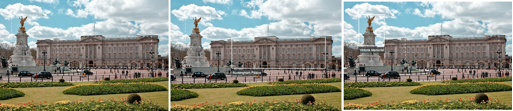
\includegraphics[width=0.5\textwidth]{images/intimage.png}
\caption{Multiple matched objects in a single query image.}
\label{fig:multiplematching}
\end{figure}

%-------------------------------
% Software architecture
%-------------------------------
\chapter{Software architecture}
\label{chpt:architecture}
While Chapter~\ref{chpt:system} outlines the processes involved with the object recognition engine, this chapter describes the practical implementation of the system including the front end web application for consumer interaction.

\begin{figure}[htb]
\centering 
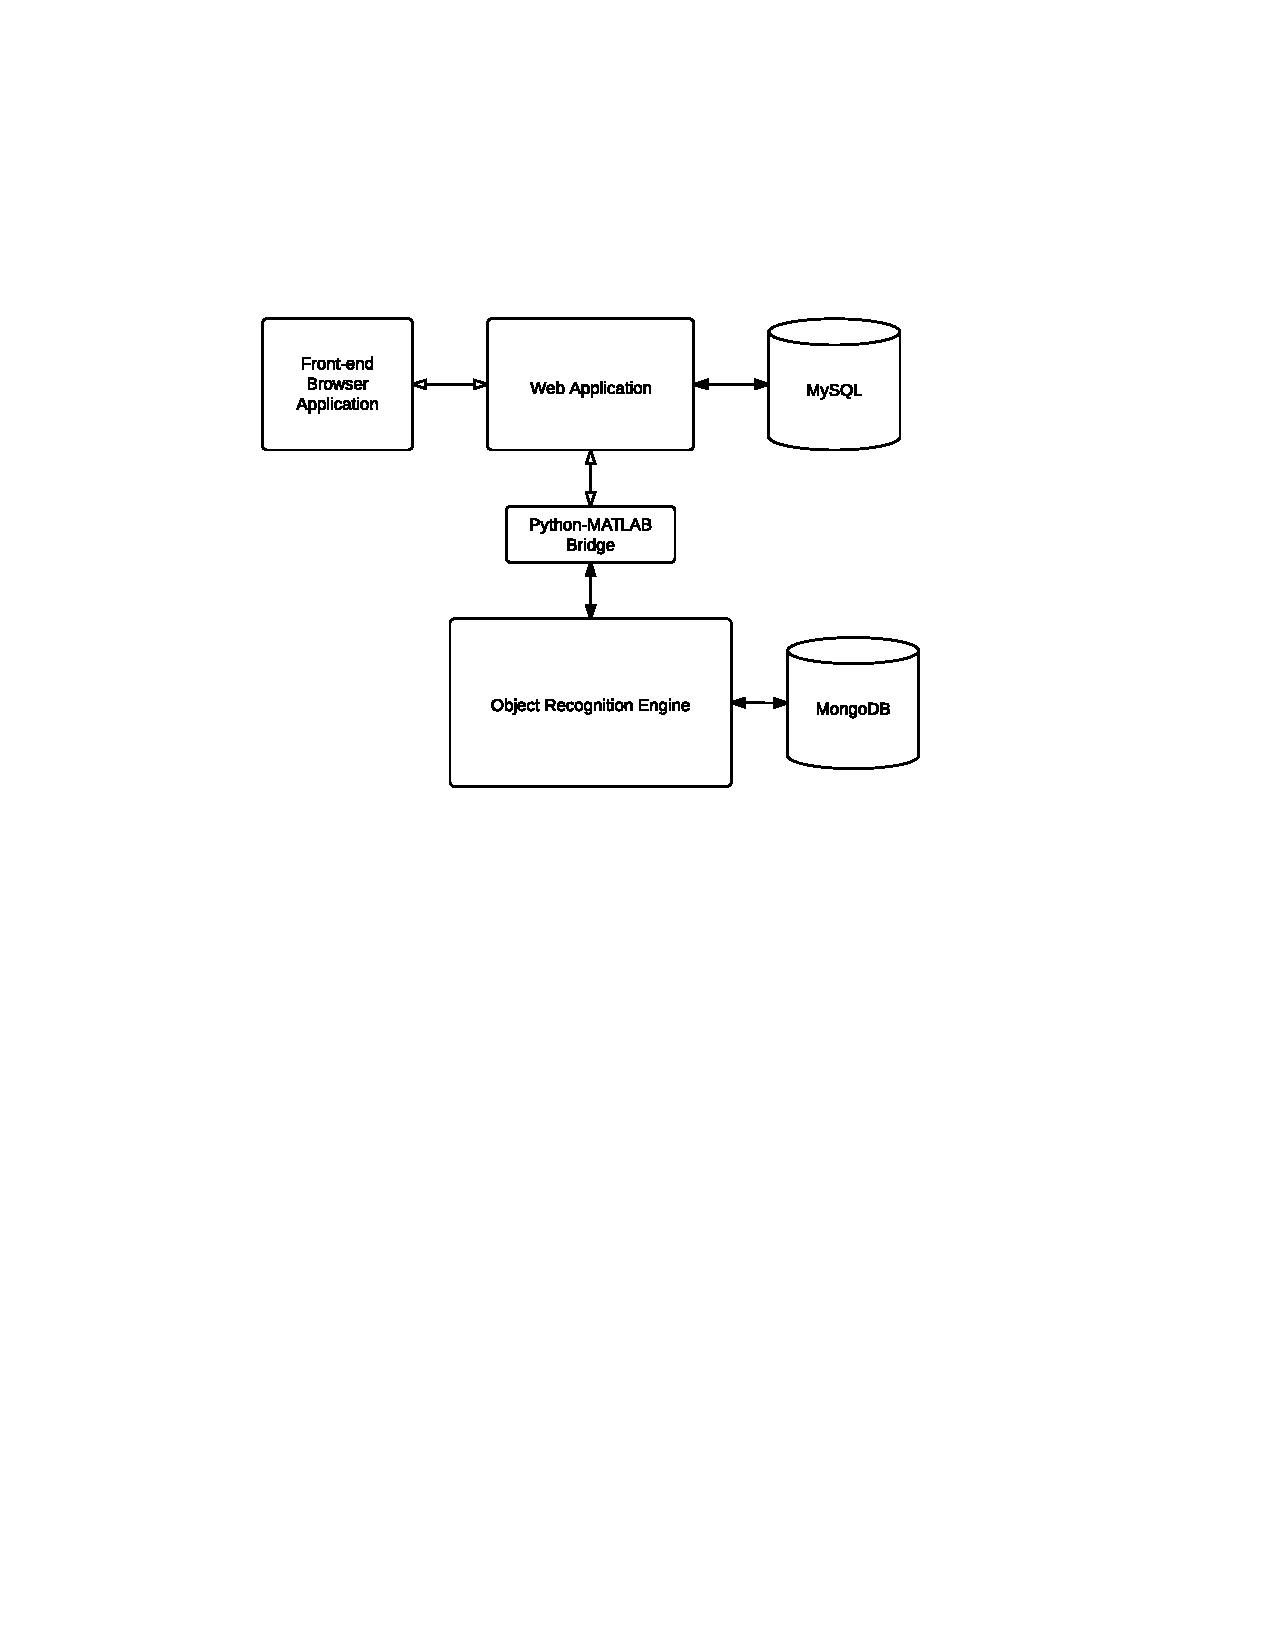
\includegraphics[width=0.7\textwidth]{images/SystemArchitecture.pdf}
\caption{An overview of the system architecture.}
\label{fig:architecture}
\end{figure}

Figure~\ref{fig:architecture} gives a holistic view of the system architecture. The solution is divided in to two separate parts: the object recognition engine and the web application. These are described in Section~\ref{sec:engine} and Section~\ref{sec:webapp} respectively. These two parts are completely independent modules by design, however they are connected via a Python-MATLAB bridge, the details of which are given in Section~\ref{sec:bridge}.

The resulting product is a web site with an intuitive user interface. A user can upload a photo, and the photo will be presented back to the user with the objects tagged.

~\section{Object Recognition Engine}
~\label{sec:engine}
The object recognition engine performs the pre-computation and recognition processes described in Chapter~\ref{chpt:system}. This is all implemented using MATLAB. MATLAB was chosen due to its ease in image manipulation, rich toolboxes, and the provided starter application was written in MATLAB.

The resulting interface is a MATLAB function \lstinline!get_objects()! that takes a single argument containing the location of the query image to recognise the objects in. The output is a structure of the object classes found and their rectangle coordinates in the query image. The function takes around 5-10 seconds to run.

~\subsection{Database}

A filesystem is used for the storage of model images (see Chapter~\ref{chpt:data}), however a working record is needed of the dataset for book keeping and quick searching. For this, MongoDB\footnote{\url{http://www.mongodb.org}} is used. 

MongoDB is a NoSQL database application that stores data in the form of documents - data structures similar to JSON objects. The data is unstructured, and provides a simple way of storing data without dealing with the complexities of tables and relationships that come with relational databases (e.g. SQL). Listing~\ref{lst:bson} shows a model image stored in the MongoDB database. The fields of the documents (i.e. \lstinline!"_id", "name", "path", "class", "size"!) are fully searchable and can be indexed for faster lookup\footnote{By deafault, the \lstinline!"_id"! field is indexed for fast lookup by ID.}. 


\linespread{1} % single line spacing
\lstset{language=Java,caption=A document representing a model image stored in MongoDB.,label=lst:bson}
\begin{lstlisting}[frame=single]
{
	"_id" : ObjectId("4f7317501b515eaa6f148c5d"),
	"name" : "1222|10_Downing_Street.jpg",
	"path" : "~/4YP/data/d_ransac/images/10_Downing_Street/1222|10_Downing_Street.jpg",
	"class" : "10_Downing_Street",
	"size" : {
		"width" : 800,
		"height" : 457
	}
}
\end{lstlisting}
\linespread{2} % double line spacing

MongoDB is run as a daemon and the directory of storage files is set to be a directory within the solutions working directory. This allows complete segmentation of each database. The daemon sets up a web server which can accept any number of connections over TCP to access the database.

The interface with MATLAB is done using the Java library provided by MongoDB\footnote{See \url{http://www.mongodb.org/display/DOCS/Java+Tutorial} for documentation.}. MATLAB has the ability to run Java inside it, so the Java MongoDB library can be consumed in a fairly natural way.

The frames, descriptors, words and histograms for the model images are stored on disk as MATLAB binary files. They are associated to the database entries via their filename which includes the ID assigned by MongoDB to the image's document. For example, for the model image \lstinline!1222|10_Downing_Street.jpg! shown in Listing~\ref{lst:bson} the frames file will be stored in the frames directory with the filename \\ \lstinline!4f7317501b515eaa6f148c5d-frames.mat!.

~\subsection{Image Processing}
The bulk of the image processing and processor intensive operations are outsourced to the VLFeat library\footnote{\url{http://www.vlfeat.org}}. VLFeat is an open source library implementing various computer vision algorithms in C. Being implemented in C means that the algorithms compute faster and more efficiently than if they were written in MATLAB. The VLFeat provides MATLAB wrappers to the functions which are use to interface with the MATLAB engine.

\lstset{language=Matlab}
To enable VLFeat, \lstinline!run vlfeat/toolbox/vl_setup! is executed on startup, after which all the VLFeat functions can be used. \lstinline!vl_sift()! is used for SIFT feature detection and descriptor computation, and \lstinline!vl_kdtreebuild()! and \lstinline!vl_kdtreequery()! are used for efficient visual word creation and retrieval.

~\subsection{Distributed Pre-computation}
The pre-computation process takes a long time to complete, as every image of the thousands in the dataset must be processed and the clustering algorithm must be run. 


~\section{Web Application}
~\label{sec:webapp}

~\section{Python-MATLAB Bridge}
~\label{sec:bridge}

%-------------------------------
% Geometric Improvements
%-------------------------------
\chapter{Geometric Improvements}
\label{chpt:geoimprovements}


%-------------------------------
% Turbo-boosting
%-------------------------------
\chapter{Turbo-boosting}
\label{chpt:turboboosting}


%-------------------------------
% Summary
%-------------------------------
\chapter{Summary}


%-------------------------------
% References
%-------------------------------
\begin{thebibliography}{99}

	\bibitem{turcot09}
		P. Turcot and D. G. Lowe.
		Better matching with fewer features: The selection of useful features in large database recognition problems
		In \emph{WS-LAVD, ICCV}, 2009.
	  
\end{thebibliography}

\end{document}